\documentclass[11pt]{article}

\usepackage{amsmath}
\usepackage{arxiv}
\usepackage{mathptmx} 
\usepackage{setspace}
\linespread{1.0} % Single spacing (default) — adjust if needed
\usepackage[utf8]{inputenc} % allow utf-8 input
\usepackage[T1]{fontenc}    % use 8-bit T1 fonts
\usepackage{hyperref}       % hyperlinks
\usepackage{url}            % simple URL typesetting
\usepackage{booktabs}       % professional-quality tables
\usepackage{amsfonts}       % blackboard math symbols
\usepackage{nicefrac}       % compact symbols for 1/2, etc.
\usepackage{microtype}      % microtypography
\usepackage{lipsum}
\usepackage{graphicx}
\usepackage{physics}
\graphicspath{ {./images/} }
% \usepackage[demo]{graphicx}
\usepackage{subcaption}
% \usepackage{lineno}
% \linenumbers

\title{ Understanding the Distribution of Fitness Effects Across Environments: exploring the Statistical Properties of Fitness Landscapes Using Fisher's Geometric Model}


\author{
 Shahnewaz Ahmed \\
  Department of Physics and Astronomy\\
Rutgers University\\
  \texttt{sa1951@rutgers.edu} \\
  %% examples of more authors
   \And
 Michael Manhart \\
  Center for Advanced Biotechnology and Medicine \\
  Rutgers University\\
  \texttt{mmanhart@rutgers.edu} \\
  \\
  %% \AND
  %% Coauthor \\
  %% Affiliation \\
  %% Address \\
  %% \texttt{email} \\
  %% \And
  %% Coauthor \\
  %% Affiliation \\
  %% Address \\
  %% \texttt{email} \\
  %% \And
  %% Coauthor \\
  %% Affiliation \\
  %% Address \\
  %% \texttt{email} \\
}
% \date{} 
\begin{document}
\maketitle
% \date{} 
\begin{abstract}
The distribution of fitness effects (DFE) is a fundamental concept in evolutionary biology; understanding the DFE is important for analyzing a variety of phenomena, including quantitative traits, complex diseases, and the evolution of antibiotic resistance. The DFE is the set of fitness effects from all spontaneous mutations accessible to an organism's genome in a specific environment. However, since environments in nature are constantly changing, understanding how the DFE varies across different environments is crucial for predicting evolutionary outcomes. In this study, we employ the Fisher Geometric Model (FGM) to explore the statistical properties of DFEs and their dependence on environmental changes. The FGM provides a theoretical framework to model fitness landscapes, where mutations are represented as random perturbations in a high-dimensional phenotypic space, and fitness is determined by the distance to an optimal phenotype.

We compare the predictions of the FGM with empirical data from a large-scale study of $\sim 3800$ gene knockout mutants of \textit{E. coli} across $\sim 100$ environments. These environments include both stress conditions (e.g., antibiotics, metals, salts) and non-stress conditions (varying carbon and nitrogen sources). By simulating DFEs under various environmental conditions, we explore whether FGM can reproduce key statistical features observed in experimental data, such as the distributions of fitness means, variances, and correlation coefficients across different environments. Our results indicate that, while the FGM successfully captures certain aspects of the data, it falls short of fully explaining the observed patterns—particularly the detailed shape of the distribution of correlation coefficients between environments. This study highlights the limitations of the FGM in describing empirical datasets and emphasizes the need for alternative or extended models to better capture the complexity of biological adaptation.
\end{abstract}


% keywords can be removed
%\keywords{First keyword \and Second keyword \and More}


\section{Introduction}
Scientists have long sought to unravel the inner workings of living organisms. In earlier decades, they made significant breakthroughs by dissecting biological systems into smaller pieces, focusing on individual elements such as genes and molecules. Today, we stand at the threshold of a new \textit{phase—one} that demands a grasp of life's full complexity. To achieve this, researchers must gather and structure enormous amounts of biological data in a consistent format, create more effective tools to retrieve and link this information, and employ advanced mathematical models to interpret it all.

One promising approach to modeling biological complexity draws inspiration from principles in physics. The concept of energy minimization, fundamental to physical systems, also finds a parallel in biological adaptation, albeit with greater complexity. In physics, objects minimize potential energy as a function of degrees of freedom (DOFs), such as a ball rolling downhill or molecules settling into low-energy configurations. Similarly, biological populations evolve toward states that optimize fitness, often visualized as movement across fitness landscapes toward peaks of maximum adaptation. By reinterpreting this landscape as a "fitness potential," where evolutionary trajectories move "downhill," we preserve the intuitive metaphor while adhering to Darwinian principles, as illustrated in Figure \ref{fig:fig1}. This framework helps bridge the conceptual gap between physics and biology, though it must be noted that biological systems introduce unique challenges due to their multidimensionality, lack of symmetry, and complexity across multiple scales \cite{agozzino2020cells, sella2005application}. Importantly, while this analogy offers valuable insights into optimization dynamics, it should not be mistaken for a deeper biological law.

\begin{figure}[t]
\begin{subfigure}{.5\textwidth}
  % \centering
  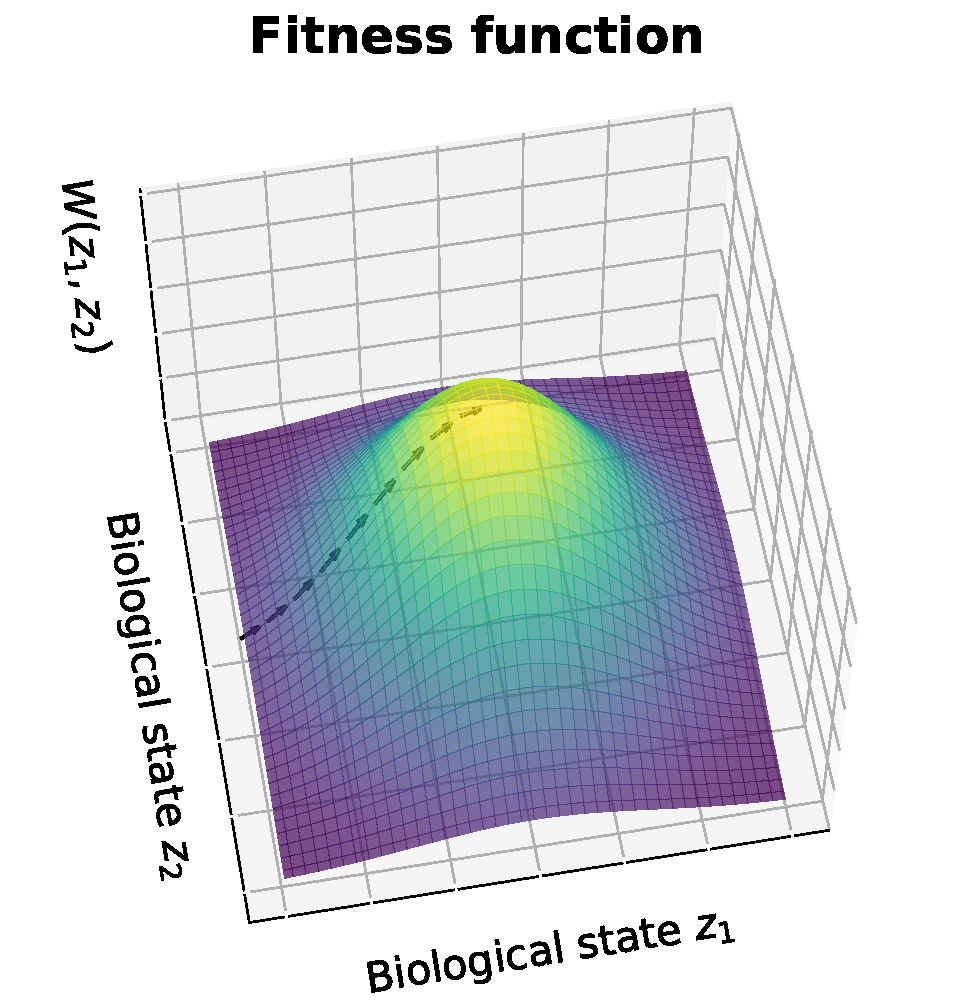
\includegraphics[width=1\linewidth]{fitness_function.pdf}
  \caption{}
  \label{fig:s1fig1a}
\end{subfigure}%
\begin{subfigure}{.5\textwidth}
  % \centering
  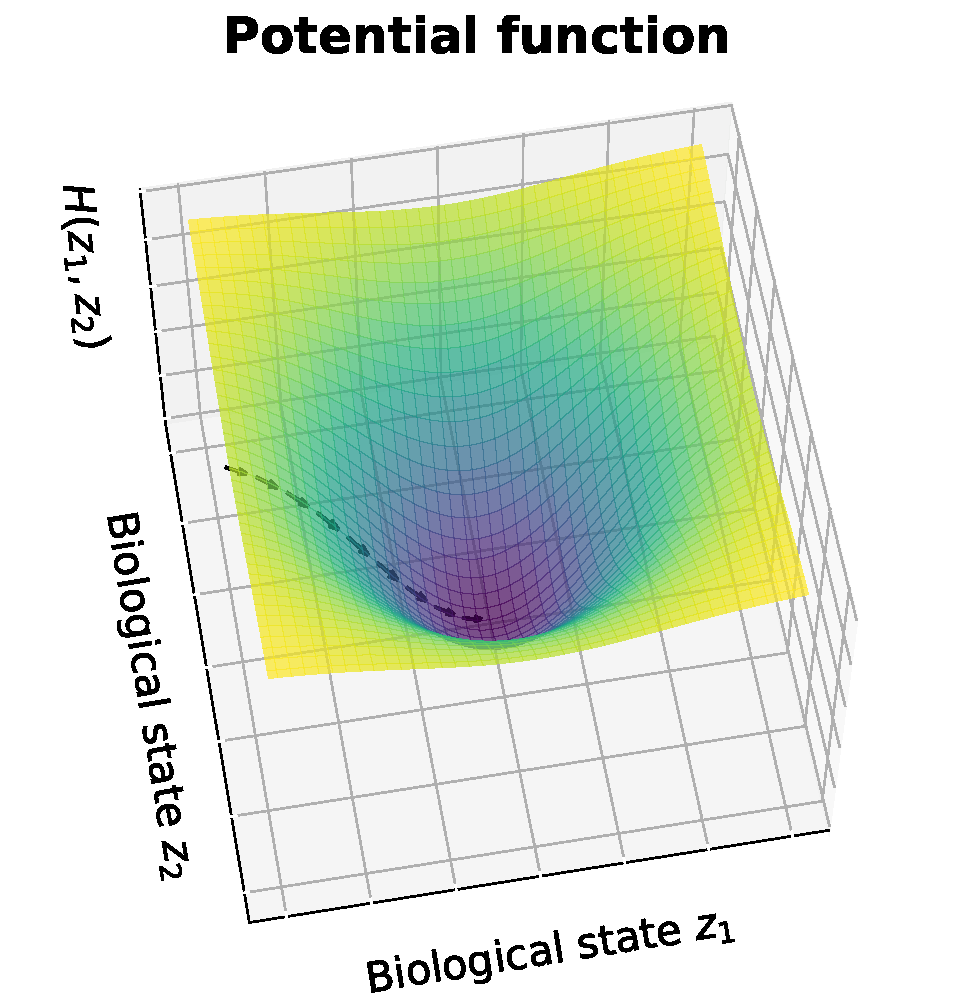
\includegraphics[width=1\linewidth]{fitness_potential.pdf}
  \caption{}
  \label{fig:s1fig1b}
\end{subfigure} \\
\caption{Evolution is often visualized as populations navigating a landscape, represented in the picture with the black arrow lines in the figures. The same process can be represented in two equivalent ways: either \ref{fig:s1fig1a} as a movement toward peaks on a fitness landscape or \ref{fig:s1fig1b} as a descent toward valleys on a landscape of potential function. }\label{fig:fig1}
\end{figure} 

Biological adaptation operates in high-dimensional spaces shaped by countless biological and ecological interactions. Even simple cells contain thousands of proteins, each with mutable amino acids, creating a vast configuration space. These landscapes are rugged, with kinetic traps that can slow adaptation, but must also contain smooth pathways to enable evolutionary progress \cite{manrubia2021genotypes, macneil2011gene}. Unlike physical systems, biological landscapes are densely packed with functional regions: minor mutations can unlock new capabilities, and promiscuous proteins allow the exploration of novel functions without losing existing ones. Such features enable both gradual refinement and rapid innovation, depending on the evolutionary context \cite{kuchner1997directed}.

Adaptation dynamics shifts as systems evolve. Early stages often involve large fitness gains from single mutations, propelling populations up steep gradients. Later stages become more complex, relying on epistatic (presence of one gene modifies the expression of another gene) interactions between multiple mutations, where the order and combination of changes determine outcomes \cite{levy2015quantitative}. Stochastic fluctuations add another layer of complexity, sometimes driving the exploration of new states and other times opposing adaptive trends \cite{tan2009emergent}. Researchers have tried to define some kind of simplified biological fitness landscape that might have mathematically tractable properties. Capturing these processes requires careful modeling choices, from selecting the right scale (molecular, cellular, or population) to defining relevant degrees of freedom and fitness metrics. Since biological optimization functions are rarely known, researchers often take a hypothesis-driven approach: proposing plausible landscape features, deriving predictions, and testing them against experimental data.

This project aims to utilize one of the earliest and simplest biological landscape models to understand how the distribution of fitness effects (DFE) of new mutations changes across different environmental conditions. DFE is a fundamental concept in evolutionary biology, characterizing the spectrum of fitness consequences arising from new mutations within a population. It offers a localized perspective on the evolutionary landscape, detailing the likelihood of different mutations becoming fixed within a population over time based on their impact on fitness. Although DFE provides a localized view of how mutations impact an organism's fitness within a specific environment, natural environments are dynamic. Therefore, to make predictions about evolutionary trajectories in the real world, it is crucial to develop or employ a simple mathematical model in order to investigate how the characteristics of the DFE, such as its mean, variance, and overall shape, are modulated by environmental change and \textit{qualitatively} compare with the experimental data.

Fisher's geometric model (FGM) seems to be a natural choice for this. In the 1930s, Robert A. Fisher, one of the three founding fathers of population genetics, proposed a geometric model of adaptation in his seminal book  "The Genetical Theory of Natural Selection" \cite{fisher1930genetical}. Although there is some empirical support for the model's prediction \cite{maclean2010diminishing, sousa2012cost}, this model is most successful at predicting the effect of epistasis on the distribution of fitness effects \cite{martin2007distributions, weinreich2013fisher}. However, the validity of this model has not being tested against a large mutational database subjected to different growth environments. Some studies did partake in observing some quantitative results from the model and comparing them with the experimental data \cite{martin2006fitness, martin2015fitness}, but those are limited to a handful of environments over different species. In this work, we investigated the prediction of this model with empirical data from a large-scale study of 3789 single-gene knockout mutants of \textit{E.coli} subjected to $101$ different environments \cite{price2018mutant}. 





\section{Description and Analysis of Experimental Data}

Among the most thoroughly researched organisms is the bacterium \textit{E. coli} K-12. Its entire genetic sequence has been mapped with remarkable precision, possibly the most detailed for any organism of its size \cite{riley2006escherichia}. This high-resolution blueprint has enabled scientists to revisit and clarify the roles of most of its genes. Given how much we already know about E. coli, and because it's a relatively simple single-celled organism, it serves as the perfect candidate for achieving a comprehensive understanding of a living system. The notion of fully deciphering E. coli isn't recent—it was even suggested as "Project K" in 1973. Back then, however, critical technologies like high-speed computing and the internet didn't yet exist \cite{crick1973project}. 

Today, high-throughput omics technologies—such as DNA sequencing (genomics), RNA sequencing (transcriptomics), and mass spectrometry (proteomics)—are revolutionizing biological and clinical research \cite{vitorino2024transforming}. In a recent large-scale study, researchers employed transposon mutagenesis (a technique where mobile genetic elements disrupt protein-coding genes) to generate mutant libraries for 32 diverse bacterial species \cite{price2018mutant}. Although transposons can change their location within the genome during initial library creation, they do not move independently after the initial library creation.

\begin{figure}
\begin{subfigure}{.5\textwidth}
  % \centering
  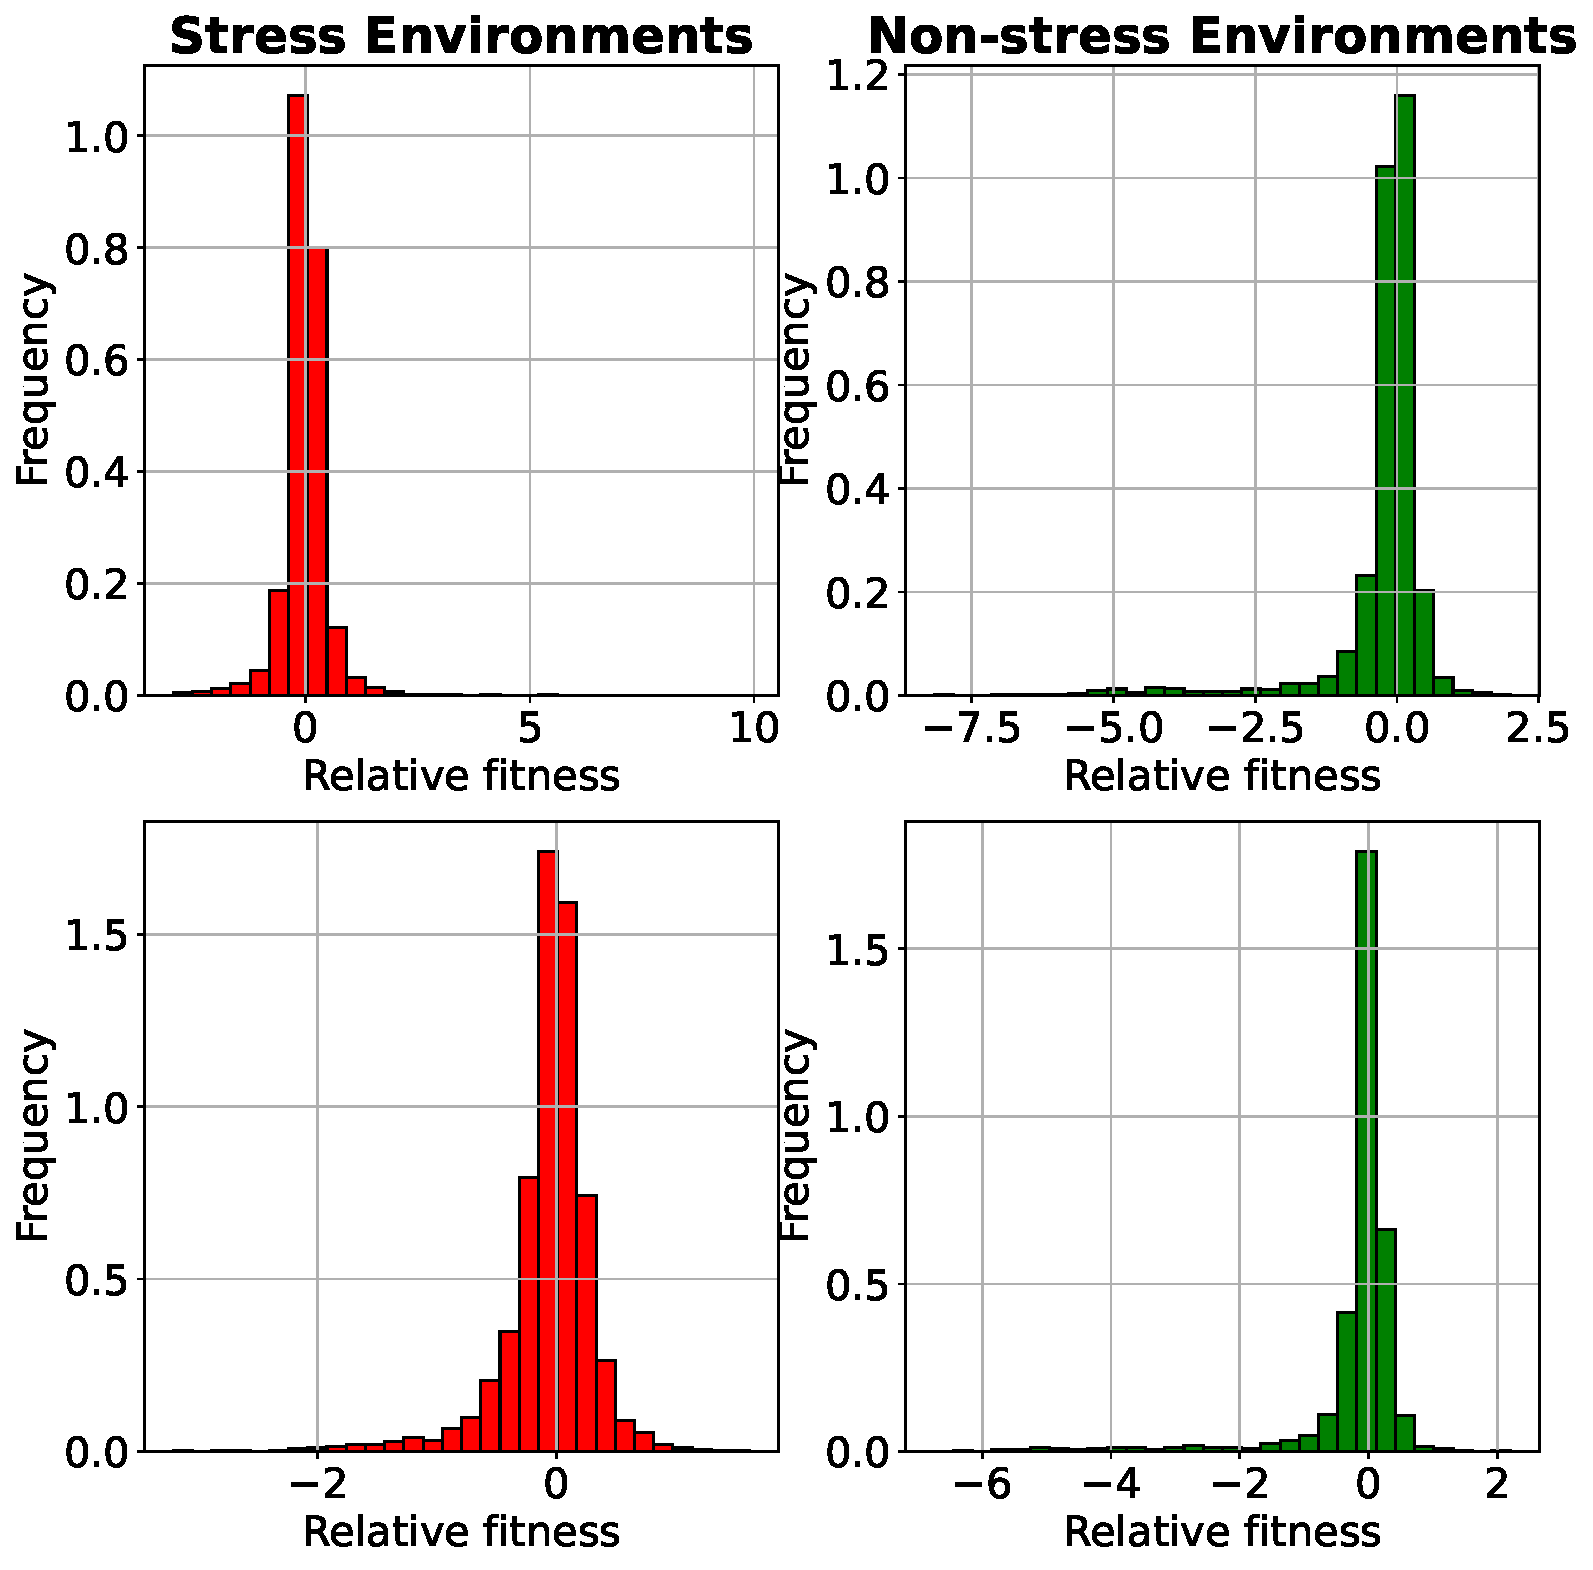
\includegraphics[width=0.95\linewidth]{exp_examples.pdf}
  \caption{}
  \label{fig:sfig3a}
\end{subfigure}%
\begin{subfigure}{.5\textwidth}
  % \centering
  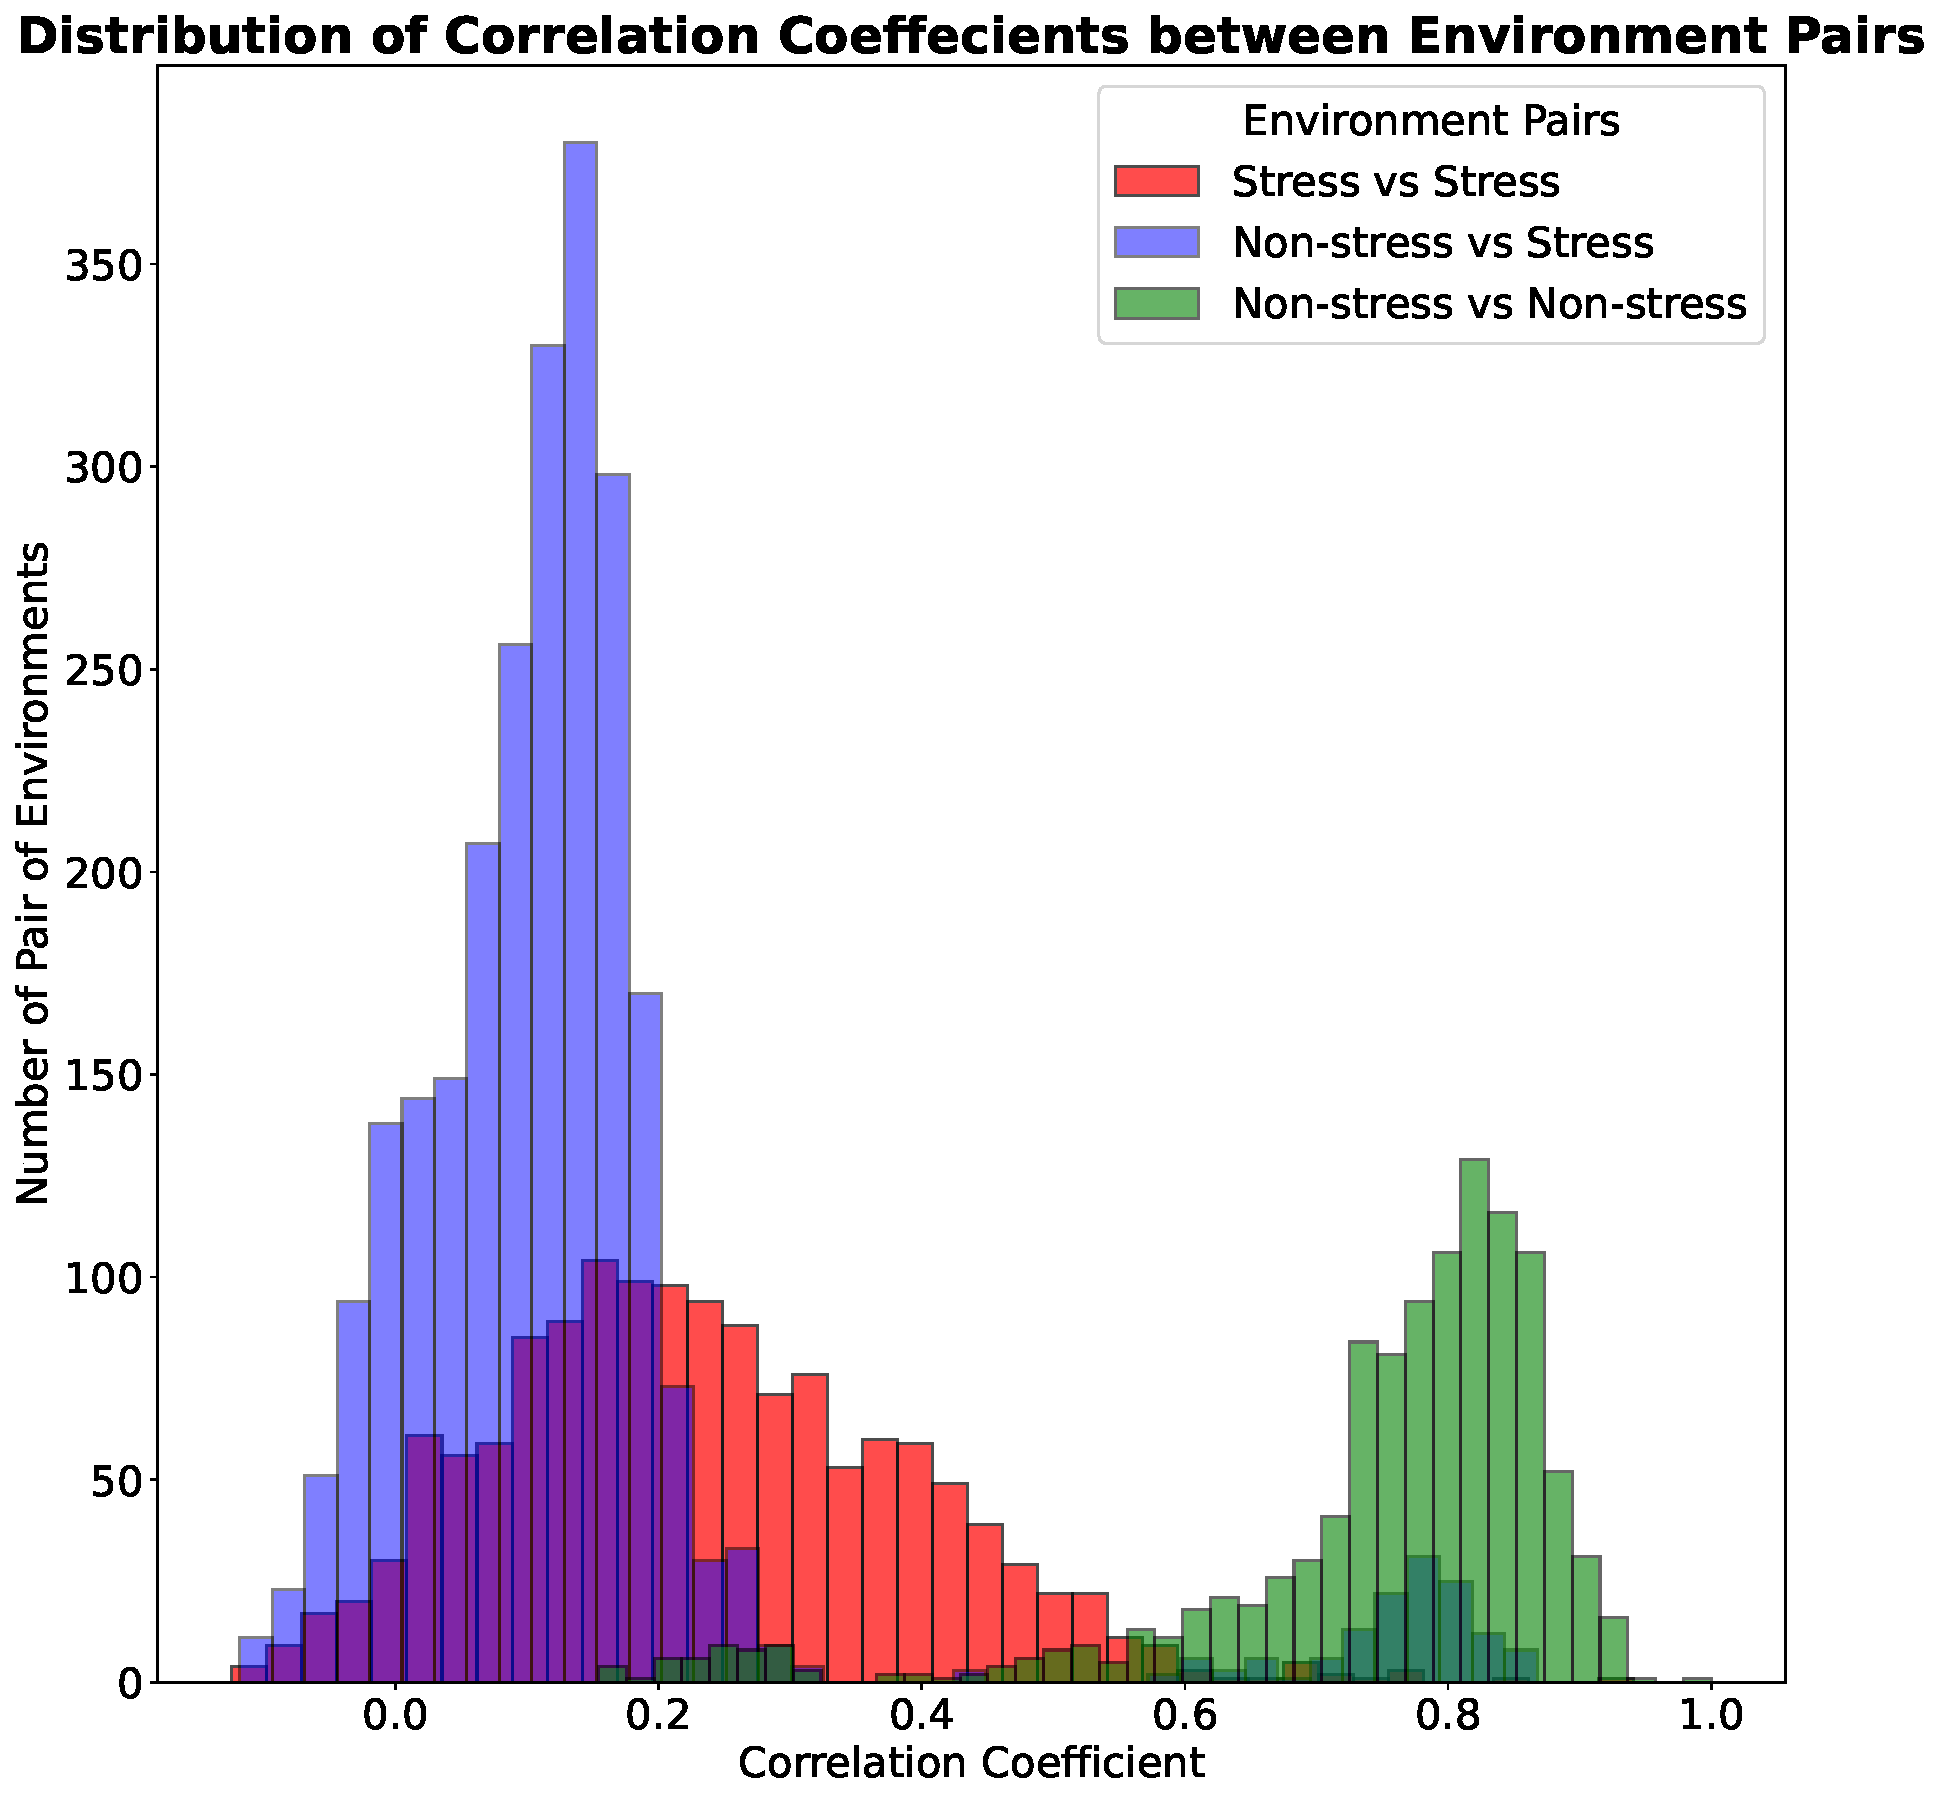
\includegraphics[width=1\linewidth]{exp_corr_samples.pdf}
  \caption{}
  \label{fig:sfig3b}
\end{subfigure} \\
\begin{subfigure}{.5\textwidth}
  % \centering
  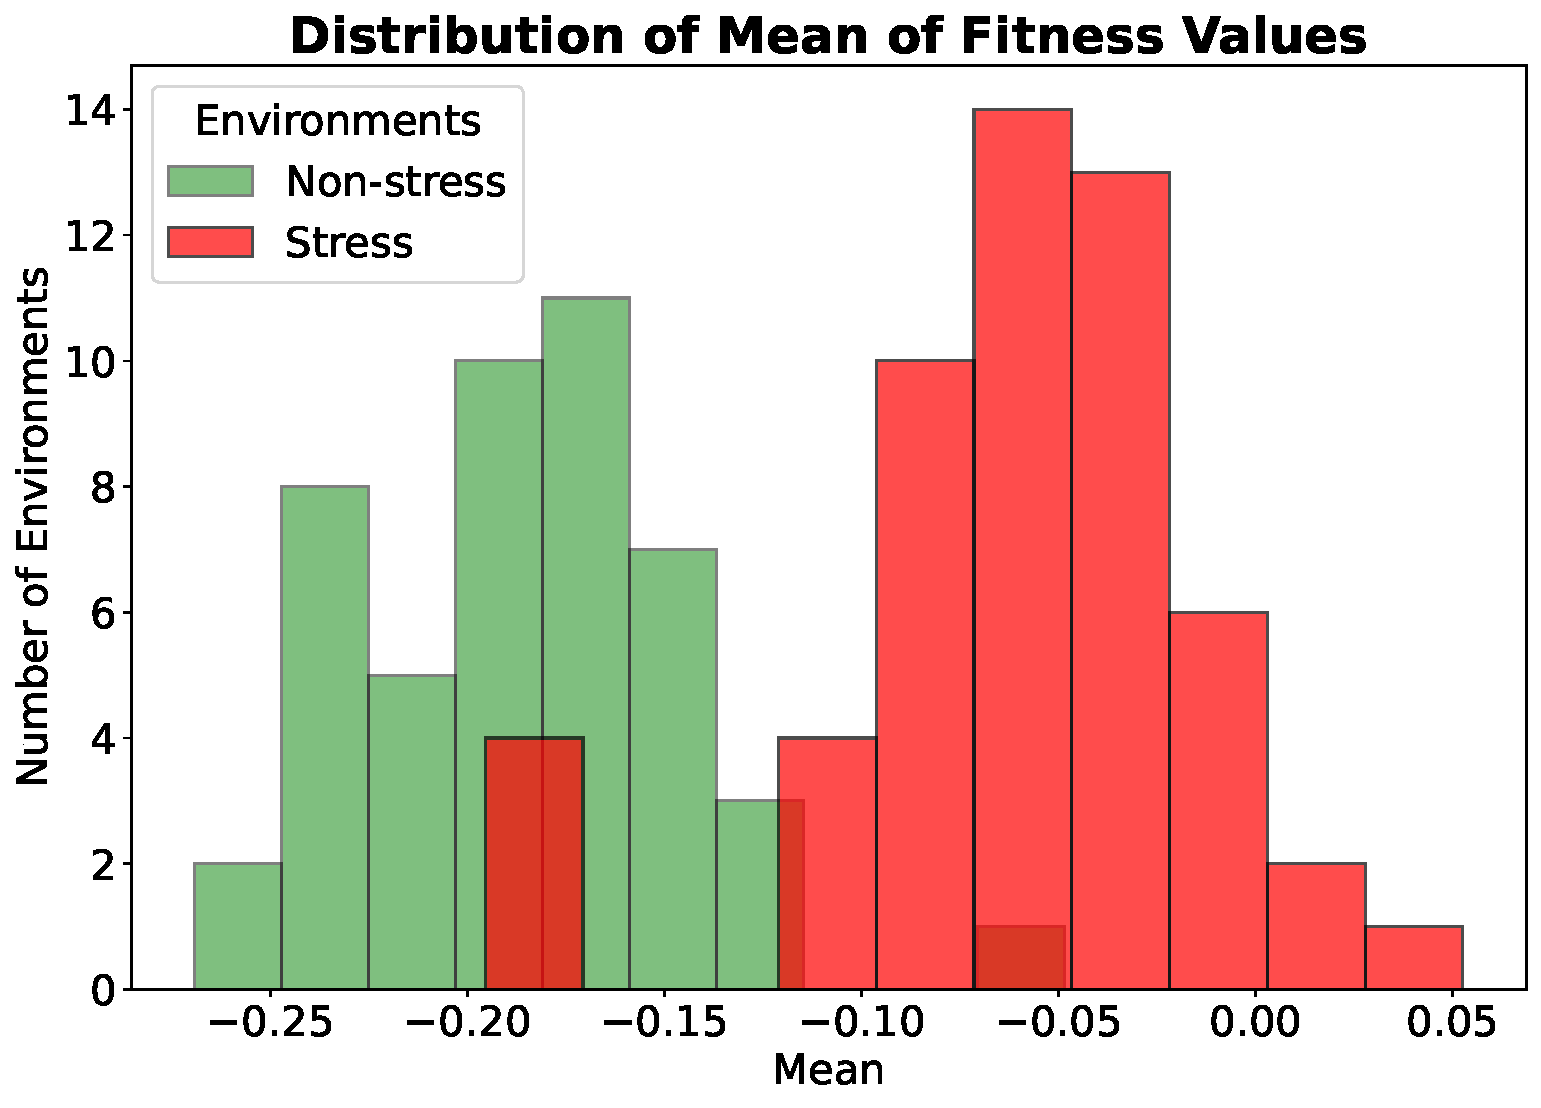
\includegraphics[width=1\linewidth]{exp_mean_samples.pdf}
  \caption{}
  \label{fig:sfig3c}
\end{subfigure}%
\begin{subfigure}{.5\textwidth}
  % \centering
  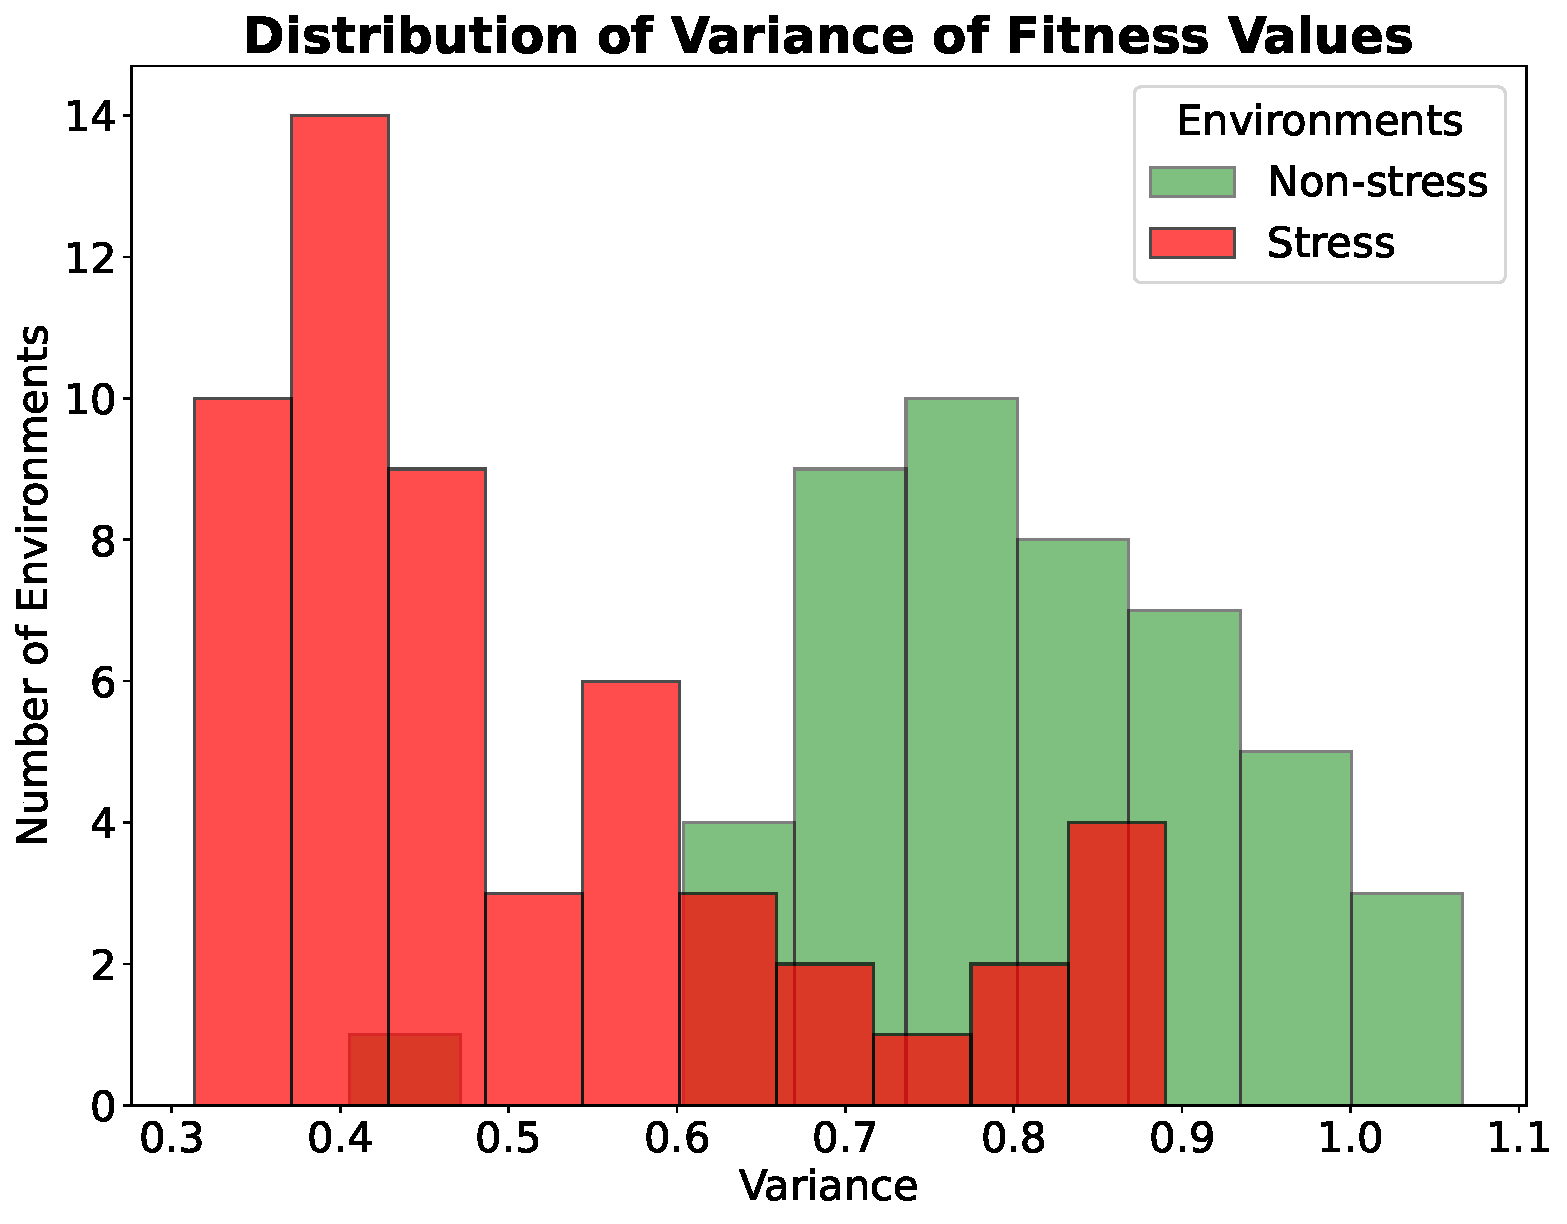
\includegraphics[width=0.92\linewidth]{exp_std_samples.pdf}
  \caption{}
  \label{fig:sfig3d}
\end{subfigure}
\caption{The four panels in Figure \ref{fig:sfig3a} illustrate sample Distributions of Fitness Effects (DFEs) for both stress and non-stress environments. These DFEs are plotted using the dataset referenced in the text. The distributions generally resemble a skewed Gaussian shape, highlighting the importance of analyzing key statistical parameters such as the mean, variance, and pairwise correlation coefficients. Figure \ref{fig:sfig3b} displays the correlation coefficient between different environment pairs. There are three possible pairings, which are highlighted separately. Figure \ref{fig:sfig3c} and \ref{fig:sfig3d} show the distribution of mean and variance, respectively, for stress and non-stress environments.  }
\label{fig:fig3}
\end{figure}


These mutants were then grown under hundreds of controlled conditions (e.g., varying nutrient availability, stressors, or environmental perturbations). Researchers first created a pool of mutant strains using randomly barcoded transposons (RB-TnSeq). Each transposon carries a unique DNA barcode and inserts randomly into the genome, allowing thousands to hundreds of thousands of mutant strains to be tracked in a particular experiment. After the mutagenesis the pool of mutant samples was recovered from the freezer in nutrient-rich media, then the cells were typically washed and sampled to establish a baseline to note the abundance at the beginning. The remaining cells were then grown under different experimental conditions. By comparing the abundance of each DNA barcode before and after the experiment, researchers determined which mutants thrived and which did not \cite{wetmore2015rapid}.

The change in abundance of mutants associated with a gene is expressed as a $\log_2$ ratio, which is the basis for the gene's fitness value. A fitness value of 0 suggests that mutants in that gene grew at rates similar to the overall population. A negative fitness value indicates that mutants were less abundant at the end, implying that the gene is important for growth or survival under those conditions. In contrast, a positive value suggests that the gene may hinder growth. To calculate gene-level fitness, the strain-level fitness values—each derived from the change in read counts of the corresponding barcodes—are averaged with a weighting system that accounts for variability in read depth. The data are also normalized so that the typical gene has a fitness value close to zero, and adjustments are made for genomic copy number variation.
\begin{align*}
    \text{Mutant fitness} &= \log_2\left( \frac{\text{abundance after}}{\text{abundance at the start}} \right) \tag{1}
\end{align*}

In order to facilitate further analyses of these mutant phenotypes and protein sequences, researchers developed a website called \href{https://fit.genomics.lbl.gov/cgi-bin/myFrontPage.cgi}{fitness browser}. From that website, we collected fitness data of \textit{E. coli} single knockout gene mutation for 3789 genes, each exposed to 101 environments, where 54 environments are labeled as stress environments and 47 environments are identified to be nutrient-rich non-stress environments. Stress environments include different antibiotic solutions, for example, Tetracycline $0.0004 \ mg/ml$, Bacitracin $0.5 \ mg / ml$, Spectinomycin $0.0125 \ mg/ml$, etc.; chemical solutions like Aluminum chloride $5 \ mM$, Cobalt chloride $0.32 \ mM$, Acetate $70 \ mM$, etc. On the other hand, Carbon-rich environments like D-Glucose, L-Fucose, Glycerol etc, Nitrogen-rich environments D-Alanine, L-Asparagine, Cytidine, etc., are considered Non-stress environments in this study. These environments are not necessarily some absolute source of Carbon and Nitrogen; rather they vary the specific compound serving as the Carbon or Nitrogen source without additional stressors.

In Figure \ref{fig:fig3}, several statistical behaviors of these fitness datasets are displayed concerning the environments. The figure \ref{fig:sfig3a} shows how the gene relative fitness would create different distributions in stress or non-stress environments. It is clear from these four figures that these distributions are highly centered around the relative fitness value of 0 and are almost evenly spread around that value. This suggests that the mean fitness values may be small for all of these environments. In contrast, stress environments exhibit small negative or even positive mean fitness values, as shown in Figure \ref{fig:sfig3a}. However, an opposite trend is observed in the variance: fitness values under stress conditions tend to have significantly lower variance—often close to zero—indicating that most mutations have similarly small effects on fitness in such environments.
% Since the environment is hostile to the ancestor or base sample, it might be similarly hostile to most mutations. Because of that, most mutation samples and the base sample have similar growth rates; hence, almost equal fitness ($\approx 0$). As a result, the value of variance is smaller compared to the non-stress environments, where the ancestor or base sample has much better growth compared to the mutated samples, and the mutation causes all sorts of possible values of fitness, resulting in an increase in the variance. 

Similarly, a strong pattern is apparent in the distribution of the correlation coefficients between the environment pairs displayed in the figure \ref{fig:sfig3b}. There is a strong correlation between non-stress environments, but stress environments exhibit a small correlation with each other and with the non-stress environments. This suggests that non-stress environments are more alike, and stress environments are very different from each other, and also not related to the non-stress ones. This behavior somewhat alludes to the Anna Karenina principle: "Happy families are all alike; every unhappy family is unhappy in its own way." A similar principle was also found in ecological risk assessment \cite{moore2001anna}. We applied this principle to guide the selection of several model parameters. The modeling framework and simulation results are detailed in the following sections.


\section{Methods}

To describe the whole premise of the model, we need to establish some concepts from biology and formalize those concepts using mathematical language for modeling. There are multiple ways of doing this, for this article, we are going to follow some standard definitions present in the literature \cite{pahujani2025complexity, tenaillon2014utility}.

\begin{itemize}
    \item \textbf{Genotype:} A genotype is the hereditary information carried by nucleic acid polymers DNA and/or RNA and passed on from a parent to its  offspring. This can be modeled using a sequence $\sigma$ with length $L$ as below:
    \begin{equation*}
        \Sigma = (\Sigma_1 , \Sigma_2, \hdots , \Sigma_L)
    \end{equation*}
    where each element of a site is taken from an alphabet $\{0, 1, 2, \hdots, a-1\}$. Each element of an alphabet is called an \textbf{allele}. 
    \item \textbf{Mutation:} In general, mutations are any form of changes in the genotype. For example one point mutations which simply change the allele at one site of a genotype $\Sigma$:
    \begin{equation*}
        \Sigma_i \to \Sigma_i' , \text{ for any } i={0, 1, \hdots, a-1}.
    \end{equation*}
    \item \textbf{Phenotype:} Phenotype of an organism is the observable characteristics or traits (e.g., plant height, color of leaves, abundance of a specific protein production inside a bacterium, etc.) produced by the interaction of the genotype and the environment. 
    \item \textbf{Fitness:} A quantity that is proportional to the mean number of viable, fertile progeny produced by some genotype. Scientists often define this quantity based on their specific experimental setups and the variables they measure. An example is provided in equation (1). For the purposes of modeling, we will define it in terms of a fitness function, which is a real-valued function of phenotype and environment.     
\end{itemize}
Fisher's geometric model is the paradigmatic representative of a phenotypic fitness landscape \cite{orr2005genetic}; it bears a close relation to the antiferromagnetic Hopfield model with random continuous pattern vectors \cite{park2020distribution}. Nevertheless, in this article, we are not going to take advantage of that relation. Hence, we will use the following sets of assumptions to define this landscape and its relationships with the genotype and phenotype of a particular organism.

\begin{figure}
\begin{subfigure}{.5\textwidth}
  % \centering
  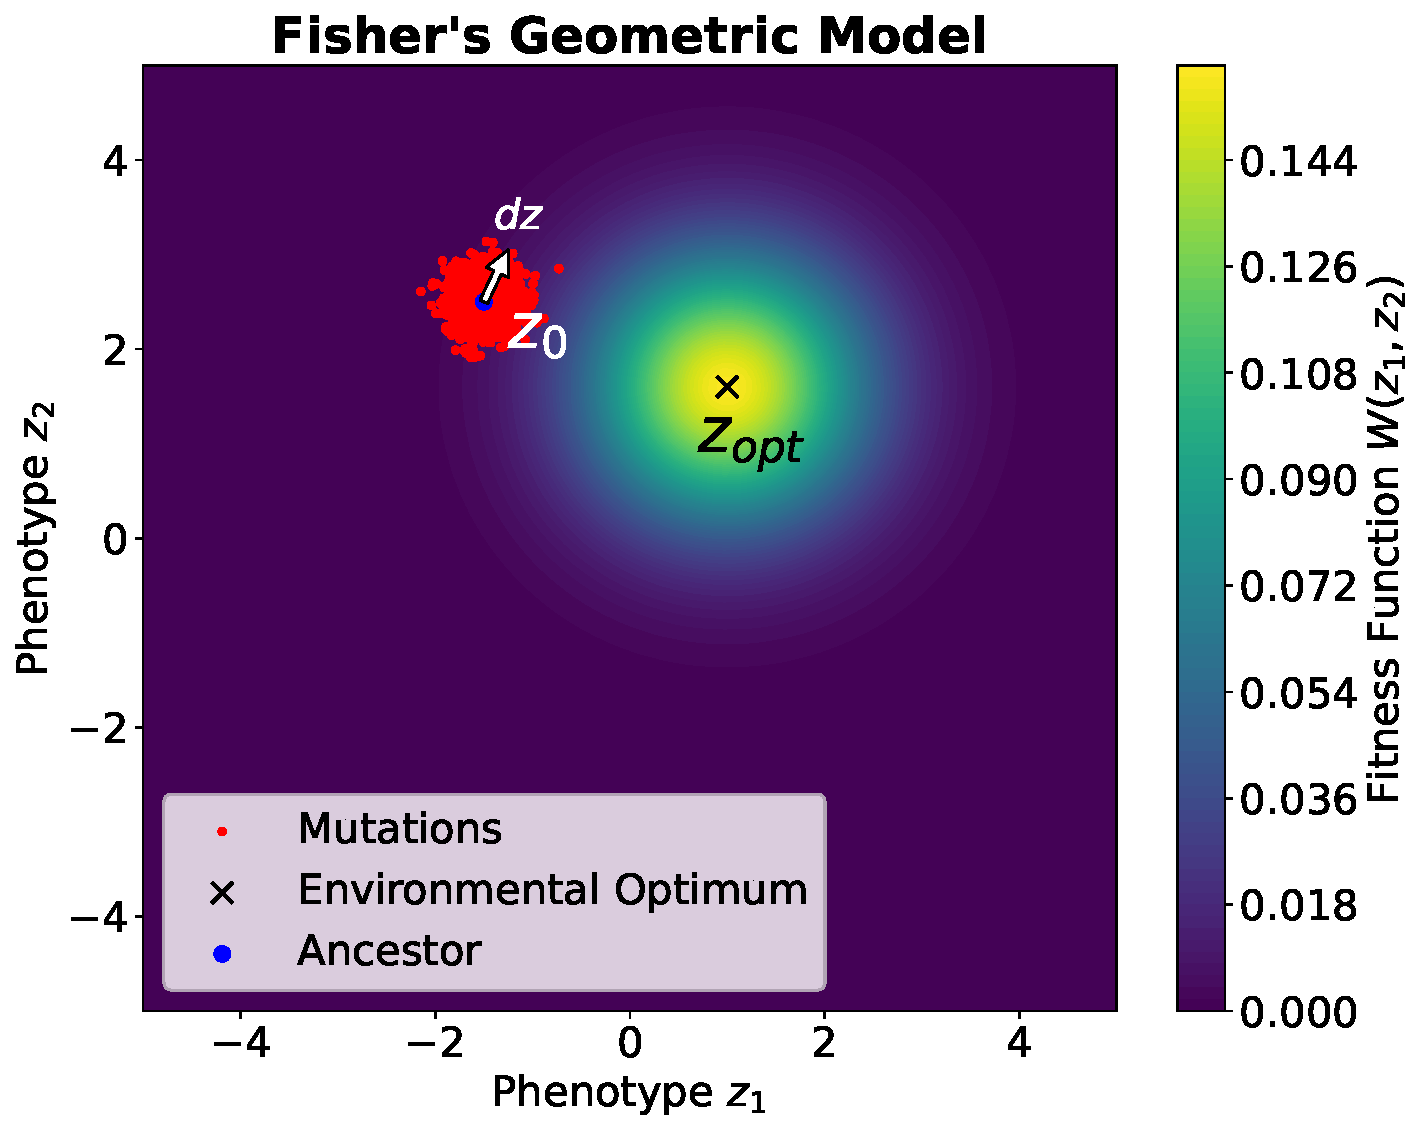
\includegraphics[width=0.90\linewidth]{Fisher_geometric_model.pdf}
  \caption{}
  \label{fig:sfig2a}
\end{subfigure}%
\begin{subfigure}{.5\textwidth}
  % \centering
  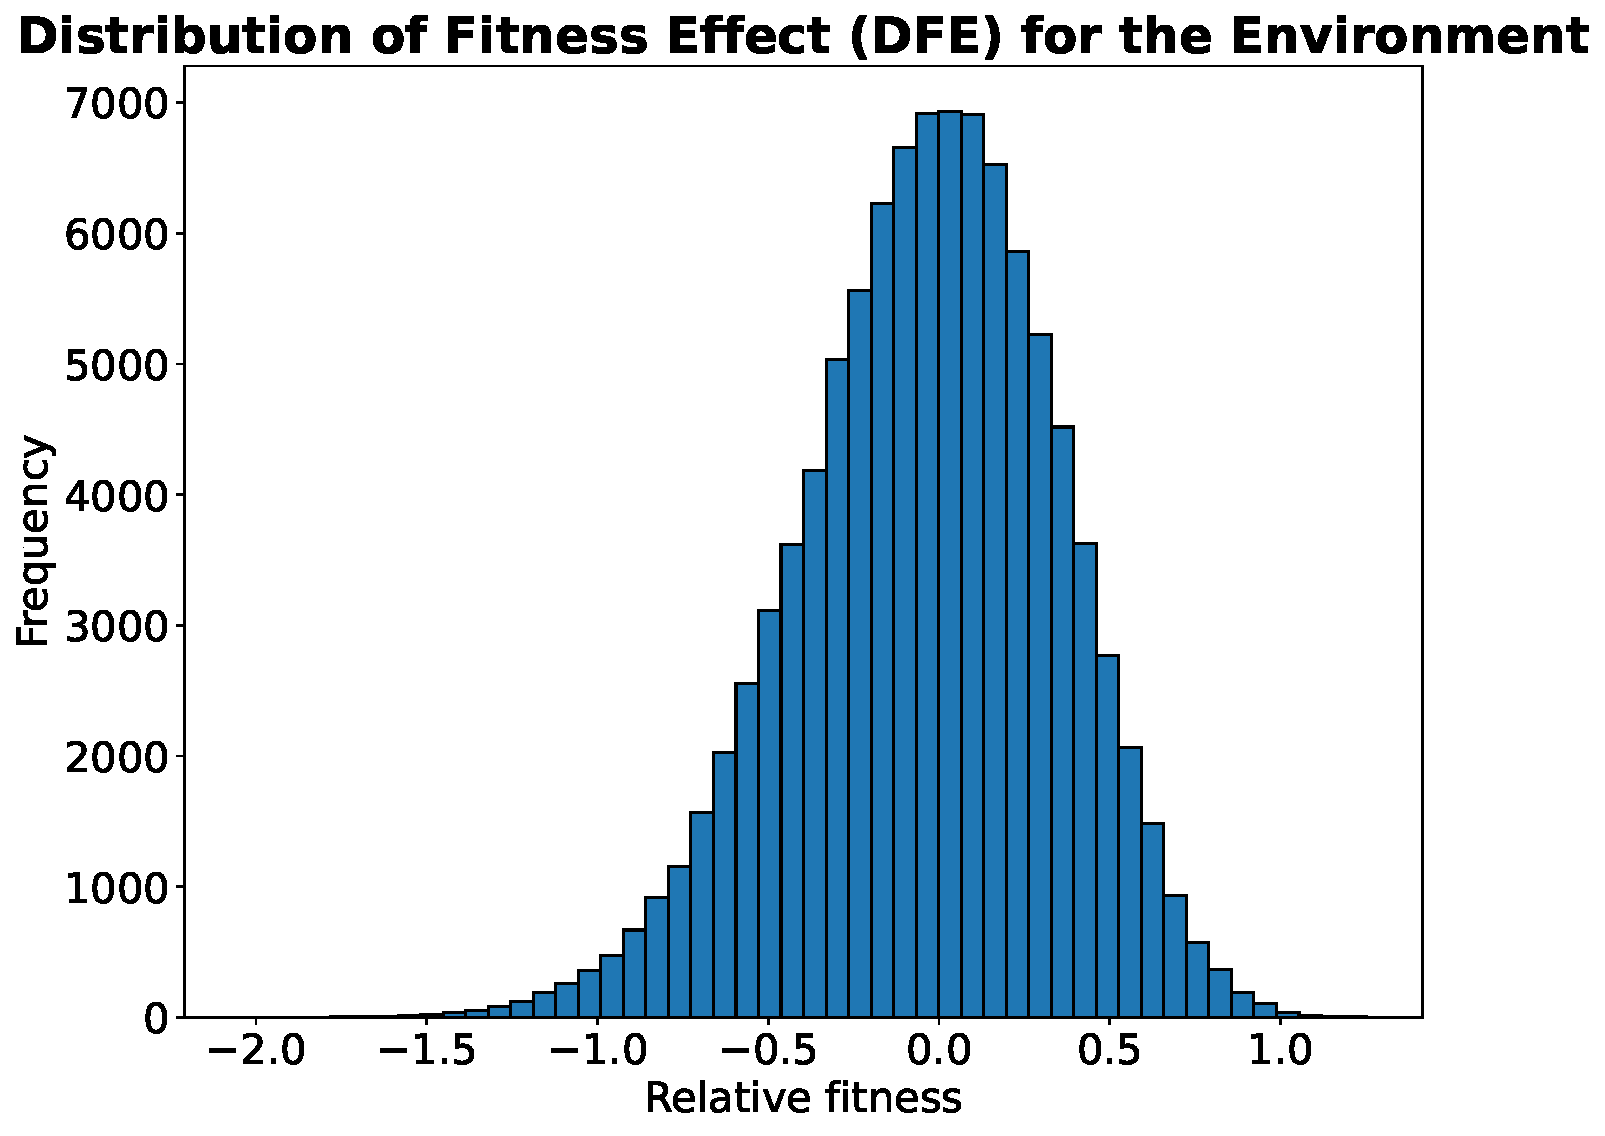
\includegraphics[width=1\linewidth]{DFEs.pdf}
  \caption{}
  \label{fig:sfig2b}
\end{subfigure}
\caption{Figure \ref{fig:sfig2a} illustrates Fisher's Geometric Model, where the ancestral species $\ket{\mathbf{z}_0}$ occupies a position in phenotype space, and the fitness function $W(z_1, z_2)$—representing a specific environment—has its optimum at $\ket{\mathbf{z}_\mathrm{opt}}$.  The red dots indicate small deviations in phenotype space resulting from mutations in the DNA of the ancestral species, and $\ket{d\mathbf{z}}$ is a corresponding vector in Phenotypic space. Figure \ref{fig:sfig2b} presents the corresponding distribution of fitness values for this scenario, commonly referred to as the Distribution of Fitness Effects (DFE). }
\label{fig:fig2}
\end{figure}

\begin{itemize}
    \item \textbf{Phenotype space:} A phenotype space is a spanned by set of \( n \) phenotypic traits \( z_i \) represented by a column vector \( \ket{\mathbf{z}} = \{z_i\}_{i \in [1,n]} \). A two-dimensional representation of the phenotype space is shown in Figure \ref{fig:fig2}. The figure also contains the fitness function.
    \item \textbf{Genotype to Phenotype Relationship:} Typically, biological organisms have a large number of genes; we can assume the genotype $\Sigma$ has a large length or $L\to \infty$. Therefore, we could ignore the discrete nature of mutation, and assign mutations that cause a phenotypic displacement \( \ket{d\mathbf{z}} = \{dz_i\}_{i \in [1,n]} \) from an initial or ancestor phenotype \( \ket{\mathbf{z}_0} \), and these vectors are distributed according to a multivariate normal distribution regardless of underlying environments $MVN(0, \sigma^2_{\mathrm{mut}} \mathbf{I}_n )$. Here, $\sigma_{\mathrm{mut}}^2$ is the variance, and $\mathbf{I}_n$ is the $n \times n$ identity matrix. This hypothesis is called "universal pleiotropy" in the literature \cite{paaby2013many}.
    \item \textbf{Phenotypic Fitness Landspace:} In this model, the fitness function is defined in terms of the phenotypic traits $z_i$. The fitness function monotonically decreases from the global maxima at $\ket{\mathbf{z}_{\mathrm{opt}}}$ isometrically, which forms nonlinear fitness isoclines by which genotype–genotype interactions emerge \cite{blanquart2014properties}. The fitness of this ancestor phenotype \( \ket{\mathbf{z}_0} \) is $W(\ket{\mathbf{z}_0}, \ket{\mathbf{z}_{\mathrm{opt}}})$ and a mutant has phenotype \( \ket{\mathbf{z}_0} + \ket{d\mathbf{z}} \) and fitness \( W( \ket{\mathbf{z}_0} + \ket{ d\mathbf{z}}, \ket{\mathbf{z}_{\mathrm{opt}}}) \). There would be one single optima in the landscape, and this hypothesis is referred as "stabilizing selection."
     
    \item \textbf{Environmental change:} The peak of $W(\ket{\mathbf{z}}, \ket{\mathbf{z}_{\mathrm{opt}}})$ defines the location of the optimal phenotype $\ket{\mathbf{z}_{\mathrm{opt}}}$, which is going to change if the environment changes without changing the shape of the fitness landscape \cite{martin2006fitness}.
    % \item \textbf{Stress and Non-stress Environments:} Following the previous assumption about the environmental changes i.e. Stress, and Non-stress environments correspond to situations where the ancestral phenotype is at a large and small distance from the optimum respectively.    
    \item \textbf{Relative Fitness or log-fitness:} The relative fitness or log-fitness function $H(\ket{\mathbf{z}}, \ket{\mathbf{z}_{\mathrm{opt}}})$ can be defined as follows:
    \begin{equation*}
        % H(\ket{\mathbf{z}}= \ket{\mathbf{z}_0} + \ket{d\mathbf{z}} , \ket{\mathbf{z}_{\mathrm{opt}}})) = \ln\left(\frac{W(\ket{\mathbf{z}_0} + \ket{d\mathbf{z}}, \ket{\mathbf{z}_{\mathrm{opt}}})}{W(\ket{\mathbf{z}_0},\ket{\mathbf{z}_{\mathrm{opt}}})} \right). \tag{2}
        H(\mathbf{z}) = \ln \left(\frac{W(\mathbf{z})}{W(\mathbf{z_0})}\right)
    \end{equation*}
    This definition agrees with the notion of the typical behavior of a potential. 
    \item \textbf{Small effect of mutation:} We will assume  \( \ket{d\mathbf{z}} \) remains small around the initial phenotype \( \ket{\mathbf{z}_{\mathrm{opt}}} \), so that \(\ln W(\ket{\mathbf{z}_0} + \ket{d\mathbf{z}},\ket{\mathbf{z}_{\mathrm{opt}}}) - \ln W(\ket{\mathbf{z}_0},\ket{\mathbf{z}_{\mathrm{opt}}})\) can be approximated by a second-order multivariate Taylor Series around \( \mathbf{z}_0 \), using Einstein's summation convention 
    \begin{align*}
    H &\approx   \frac{\partial \ln W(\ket{\mathbf{z}_0}, \ket{\mathbf{z}_{\mathrm{opt}}})}{\partial z_i} dz_i  + \frac{1}{2}  \frac{\partial^2 \ln W(\ket{\mathbf{z}_0}, \ket{\mathbf{z}_{\mathrm{opt}}})}{\partial z_i \partial z_j} dz_i dz_j + o[dz^3]. \tag{3}
    \end{align*} 
    % The rationale for this definition can be understood using the idea of relative fitness. \( W \) is the absolute fitness, but the effect of mutation accumulation on relative fitness \( H \), that is, on the distribution of the fitness deviation of mutations relative to the initial genotype. This deviation for mutant with phenotype \( \mathbf{z}_0 + d\mathbf{z} \) is \[ dw = \frac{W(\ket{\mathbf{z}_0} + \ket{d\mathbf{z}},\ket{\mathbf{\zeta_0}}) - W(\ket{\mathbf{z}_0},\ket{\mathbf{z}_{\mathrm{opt}}})}{W(\ket{\mathbf{z}_0},\ket{\mathbf{z}_{\mathrm{opt}}})}, \] which is the selection coefficient of the mutant line relative to its wild-type ancestor. If the deviations remain small, the effect of \( \ket{d\mathbf{z}} \) on relative fitness approximately equals its effect on absolute log-fitness \( \ln[W(\mathbf{z})] \) (denoted in \( W(\mathbf{z}) \)):\[ dw \approx \ln(1 + dw) = \ln W(\ket{\mathbf{z}_0} + \ket{d\mathbf{z}}, \ket{\mathbf{z}_{\mathrm{opt}}}) - \ln W(\ket{\mathbf{z_0}},\ket{\mathbf{z}_{\mathrm{opt}}}). \]
    
\end{itemize}

% A straightforward way to evaluate the effect of the environment on the distribution of mutation fitness effects \( f(s) \), is to consider fitness landscape models, similar to Fisher's (1930) geometric model, whereby the fitness of a given phenotype falls off with the phenotypic distance to an optimum determined by the environment. Assuming a distribution of mutational effects on phenotypic traits, this approach provides a natural way to predict \( f(s) \) at a given distance from the phenotypic optimum (Orr 2000; Welch and Waxman 2003). 

% We can model a phenotype as a set of \( n \) phenotypic traits \( z_i \) represented by a column vector \( \mathbf{z} = \{z_i\}_{i \in [1,n]} \), with fitness given by an arbitrary (twice differentiable) fitness function \( W(\mathbf{z}) \). Each MA line accumulates mutations causing a phenotypic displacement \( d\mathbf{z} = \{dz_i\}_{i \in [1,n]} \) from an initial phenotype \( \mathbf{z}_0 \). 

\section{Results}

The evolutionary fate of a population depends critically on the effects of individual mutations on organismal fitness. Mutations are broadly categorized as either deleterious or beneficial. To mathematically characterize these effects, one must consider the distribution of fitness values across all possible mutations, commonly referred to as the Distribution of Fitness Effects (DFE). Although determining the exact shape of the DFE is challenging, valuable insights can still be gained by examining key statistical parameters such as the mean, variance, and correlation coefficients. Using equation (3), we can compute the mean \(  M \)  and variance \(  V \)  of \( H \) over mutants \( \ket{d\mathbf{z}} \). In literature, it has been observed that just an unbiased assumption could work, and there is no clear trend expected or observed for the effect of mutations on, for example, morphological traits \cite{martin2006general}. According to the genotype and phenotype relation in our model assumption $\ket{d\mathbf{z}}$ has a multivariate distribution, we can deduce that mutation effects on phenotypic traits \( (\ket{\mathbf{z}}) \) are unbiased, \( E[dz_i] = 0 \). 

\textbf{Mean:} Now, keeping only terms up to the second order in \(dz\), equation (3) yields the mean
\begin{align}
 M = E(H) &\approx \frac{1}{2} \frac{\partial^2 \ln W(\ket{\mathbf{z}_0}, \ket{\mathbf{z}_{\mathrm{opt}}})}{\partial z_i \partial z_j} E[dz_i dz_j] + o[E[dz^3]], \tag{4} 
\end{align}
From equation (4), the average relative fitness effect of mutations or \( M \) depends on the local curvature of the log-fitness function at the optimum, \(\partial^2 \ln W(\ket{\mathbf{z}_0}, \ket{\mathbf{z}_{\mathrm{opt}}})/\partial z_i \partial z_j\). Indeed, symmetrical variation in \(dz\) can just introduce a bias in \(H\) if the phenotype-fitness relationship \(\ln W(\ket{\mathbf{z}_0}, \ket{\mathbf{z}_{\mathrm{opt}}}) \) is nonlinear. 
Now suppose, the logarithmic fitness is concave around \(\ket{\mathbf{z}_0}\), that is, \( J = \big[ \partial^2 \ln W(\ket{\mathbf{z}_0}, \ket{\mathbf{z}_{\mathrm{opt}}})/\partial z_i \partial z_j \big]\) is a negative semi-definite matrix, then the mutations are deleterious on average (\( M \leq 0\)). 

This claim can be proven by the first, utilizing the fact that the Hessian matrix \(    J = \lambda_i \ket{\Lambda_i}\bra{\Lambda_j},
\) can be decomposed into its eigenvalues $\lambda_i<0$ ($\forall i = 1, \hdots, n$) and corresponding eigenvectors $\ket{\Lambda_i}$,
and given a vector,  $\ket{dz} = [dz_1, \hdots, dz_n]^T$ we can write
\begin{align*}
    \frac{1}{2}  \frac{\partial^2 \ln W(\ket{\mathbf{z}_0}, \ket{\mathbf{z}_{\mathrm{opt}}})}{\partial z_i \partial z_j} dz_i dz_j = \frac{1}{2} \bra{dz} J \ket{dz} = \frac{1}{2} \lambda_i |
   \braket{dz}{\Lambda_i}|^2 \leq 0.
\end{align*}
Combining with eq(4) we get,
\begin{align*}
    M &\approx E\left[ \frac{1}{2} \frac{\partial^2 \ln W(\ket{\mathbf{z}_0}, \ket{\mathbf{z}_{\mathrm{opt}}})}{\partial z_i \partial z_j} dz_i dz_j\right] + o[E[dz^3]] \leq 0.
\end{align*}
From this result, we can imply that if $\ket{\mathbf{z}_0}$ is close to the global optima $\ket{\mathbf{z}_{\mathrm{opt}}}$ where the log-fitness may be more concave than other places, the mean $M$ is going be more negative, hence more deletarious.  On the other hand, since \(E[dz_i] = E[dz_j] = 0\), the terms \(E[dz_i dz_j]\) are the variances and covariances of the effects of mutation accumulation on the underlying phenotypic traits. Furthermore, since $dz$ distributed according to $MVN(0, \sigma^2_{\mathrm{mut}} \mathbf{I}_n )$, \[E[dz_i dz_j] = \delta_{ij}\sigma^2_{\mathrm{mut}}.
\] This value quantify globally how and how much mutation accumulation affects the phenotype distribution among mutants. Now applying  this multivariate normal distribution and the isotropic fitness function assumption i.e., $W(\ket{\mathbf{z}_0},\ket{\mathbf{z}_{\mathrm{opt}}}) =  W(||\mathbf{z}_0 - \mathbf{z}_{\mathrm{opt}} ||)$ for the mutation vectors assumption, mean $M$ becomes
    \begin{align*}
        M \approx& \ \frac{1}{2} \frac{\partial^2 \ln W(\ket{\mathbf{z}_0}, \ket{\mathbf{z}_{\mathrm{opt}}})}{ \partial z_i \partial z_j} \delta_{ij}\sigma_{\mathrm{mut}}^2 + o[E[dz^3]] \\
        % \approx& \ \frac{ \sigma_{\mathrm{mut}}^2}{2} \frac{\partial}{\partial z_i} \Big( \frac{\partial \ln W(||\mathbf{z}_0 - \mathbf{z}_{\mathrm{opt}} ||)}{\partial(||\mathbf{z}_0 - \mathbf{z}_{\mathrm{opt}} ||)} \frac{(z_{0,i}-\zeta_{0,i})}{||\mathbf{z}_0 - \mathbf{z}_{\mathrm{opt}} ||} \Big) + o[E[dz^3]] \\
        % \approx& \ \frac{ \sigma_{\mathrm{mut}}^2}{2}  \Big( \frac{\partial \ln W(||\mathbf{z}_0 - \mathbf{z}_{\mathrm{opt}} ||)}{\partial(||\mathbf{z}_0 - \mathbf{z}_{\mathrm{opt}} ||)} \frac{\delta_{ii}}{||\mathbf{z}_0 - \mathbf{z}_{\mathrm{opt}} ||} \\
        % & \quad \quad + \frac{(z_{0,i}-\zeta_{0,i})(z_{0,i}-\zeta_{0,i})}{||\mathbf{z}_0 - \mathbf{z}_{\mathrm{opt}} ||}\frac{\partial}{\partial (||\mathbf{z}_0 - \mathbf{z}_{\mathrm{opt}} ||)} \Big(\frac{\partial \ln W(||\mathbf{z}_0 - \mathbf{z}_{\mathrm{opt}} ||)}{\partial(||\mathbf{z}_0 - \mathbf{z}_{\mathrm{opt}} ||)} \frac{1}{||\mathbf{z}_0 - \mathbf{z}_{\mathrm{opt}} ||} \Big) \Bigg) + o[E[dz^3]]
        \\  \approx& \ \frac{ \sigma_{\mathrm{mut}}^2}{2}   \Big( \frac{\partial^2 \ln W(||\mathbf{z}_0 - \mathbf{z}_{\mathrm{opt}} ||)}{\partial(||\mathbf{z}_0 - \mathbf{z}_{\mathrm{opt}} ||)^2} + \frac{n-1}{||\mathbf{z}_0 - \mathbf{z}_{\mathrm{opt}} ||} \frac{\partial \ln W(||\mathbf{z}_0 - \mathbf{z}_{\mathrm{opt}} ||)}{\partial(||\mathbf{z}_0 - \mathbf{z}_{\mathrm{opt}} ||)}   \Big) + o[E[dz^3]].  \tag{5}
    \end{align*}
Here, the last line is derived using an identity related to transformation of the $N$-dimensional Laplace operator from cartesian to spherical coordinates.

\textbf{Variance}: As for the variance
\begin{align*}
    V &= E[H^2] - M^2  \approx  E\left[\frac{\partial \ln W(\ket{\mathbf{z}_0}, \ket{\mathbf{z}_{\mathrm{opt}}})}{\partial z_i} \frac{\partial \ln W(\ket{\mathbf{z}_0}, \ket{\mathbf{z}_{\mathrm{opt}}})}{\partial z_j} dz_i dz_j + o[dz^3]\right] - M^2 \\
    & \approx \frac{\partial \ln W(\ket{\mathbf{z}_0}, \ket{\mathbf{z}_{\mathrm{opt}}})}{\partial z_i} \frac{\partial \ln W(\ket{\mathbf{z}_0}, \ket{\mathbf{z}_{\mathrm{opt}}})}{\partial z_j} E[dz_i dz_j] + o[E[dz^3]]. \tag{6}
\end{align*}
Let's impose the multivariate normal distribution for the mutation vectors. As a consequence, we get,
    \begin{align*}
        V & \approx  \Big( \frac{\partial \ln W(\ket{\mathbf{z}_0}, \ket{\mathbf{z}_{\mathrm{opt}}})}{\partial z_i} \frac{\partial \ln W(\ket{\mathbf{z}_0}, \ket{\mathbf{z}_{\mathrm{opt}}})}{\partial z_i} \Big) \sigma_{\mathrm{mut}}^2 + o[E[dz^3]]. \tag{7}
    \end{align*}
% This approximation shows that both the average and variance of the relative fitness of MA lines can be decomposed into two parts reflecting the genotype-phenotype relationship (\(E[dz_i dz_j]\)), and the phenotype-(log)fitness relationship (derivatives of \(\ln W(\ket{\mathbf{z}_0}, \ket{\mathbf{z}_{\mathrm{opt}}})\) at phenotype \(\ket{\mathbf{z}_0}\)).

 % Equations (4,5) shows that the mean and variance of mutation effects are both proportional to \(E[dz_i dz_j]\): both \( M\) and \( V\) scale with the amount of phenotypic change produced by mutation accumulation.

% It is evident from the previous discussion that $H(\mathbf{z})$ describes how phenotypic changes (\(dz_i\)) translate into relative fitness changes (\(dw\)) in a given environment.
% \begin{itemize}
    % \item
    % Later, we will assume a constant curvature, which results in a Gaussian function for the fitness function.  
  
    % \item
    The mutational variance in relative fitness (\( V\)) is proportional to the product of first derivatives of \(\ln W(\ket{\mathbf{z}_0}, \ket{\mathbf{z}_{\mathrm{opt}}})\) taken at \(\ket{\mathbf{z}_0}\). This result is intuitively simple: the variance in the underlying phenotypic traits (\(z_i\)) translates into the variance in fitness according to the local slope of the fitness function (to \(\partial \ln W(\ket{\mathbf{z}_0}, \ket{\mathbf{z}_{\mathrm{opt}}})/\partial z_i\)) irrespective of its sign (hence the square). 

    Now, if the fitness function \( W\) monotonic with the distance to the optimum \(||{z_0}-{\zeta_0}||\). From which we essentially arrive at the following formula from equation (7)
    \begin{align*}
        V \approx& \Bigg(\frac{\partial \ln W(||\mathbf{z}_0 - \mathbf{z}_{\mathrm{opt}} ||)}{\partial(||\mathbf{z}_0 - \mathbf{z}_{\mathrm{opt}} ||)} \sigma_{\mathrm{mut}} \Bigg)^2 + o[E[dz^3]] \tag{8}
    \end{align*}
    
    % \item 
\textbf{Correlation coefficient:} If we consider two different environments with two different optimum $\ket{\mathbf{z}_{\mathrm{opt}}}, \ket{\mathbf{z'}_{\mathrm{opt}}}$, with two fitness landscapes $W(\ket{\mathbf{z}_0}, \ket{\mathbf{z}_{\mathrm{opt}}})$ and $W(\ket{\mathbf{z}_0}, \ket{\mathbf{z'}_{\mathrm{opt}}})$ respectively, we can calculate the Pearson's correlation coefficients,
    \begin{align*}
        \rho_{H,H'} = \frac{E(HH')-E(H)E(H')}{\sqrt{E(H^2)-E(H)^2}\sqrt{E(H'^2)-E(H')^2}} 
    \end{align*}
    where $H, H'$ are the log-fitness for mutations with respect to $\ket{\mathbf{z}_0}$ for the environments with phenotypic optimums at $\ket{\mathbf{z}_{\mathrm{opt}}}, \ket{\mathbf{z'}_{\mathrm{opt}}}$ respectively. We can rewrite the formula of the correlation coefficients $\rho_{H,H'}$ in terms of means and variances as follows:
    \begin{align*}
        \rho_{H,H'} = \frac{E(HH')-MM'}{\sqrt{V V'}}.
    \end{align*}
    Now, we can focus on $E[HH']$ by rewriting it more explicitly,
    \begin{align*}
        E[HH'] \approx& \ \ E\Bigg[\Big( \frac{\partial \ln W(\ket{\mathbf{z}_0}, \ket{\mathbf{z}_{\mathrm{opt}}})}{\partial z_i} dz_i  + \frac{1}{2}  \frac{\partial^2 \ln W(\ket{\mathbf{z}_0}, \ket{\mathbf{z}_{\mathrm{opt}}})}{\partial z_i \partial z_j} dz_i dz_j + o[dz^3] \\
        & \quad \times\Big( \frac{\partial \ln W(\ket{\mathbf{z}_0},\ket{\mathbf{z'}_{\mathrm{opt}}})}{\partial z_p} dz_p  + \frac{1}{2} \frac{\partial^2 \ln W(\ket{\mathbf{z}_0}, \ket{\mathbf{z'}_{\mathrm{opt}}})}{\partial z_p \partial z_q} dz_p dz_q + o[dz^3]\Big)\Bigg] \\
        \approx& \ \frac{\partial \ln W(\ket{\mathbf{z}_0}, \ket{\mathbf{z}_{\mathrm{opt}}})}{\partial z_i} \frac{\partial \ln W(\ket{\mathbf{z}_0},\ket{\mathbf{z'}_{\mathrm{opt}}})}{\partial z_j}  E[dz_i dz_j] + o[E[dz^3]].
    \end{align*}
    Next, we can impose $ E[dz_i dz_j] = \delta_{ij} \sigma_{\mathrm{mut}}^2$, which gives us
    \begin{align*}
         E[HH'] \approx&\  \frac{\partial \ln W(\ket{\mathbf{z}_0}, \ket{\mathbf{z}_{\mathrm{opt}}})}{\partial z_i} \frac{\partial \ln W(\ket{\mathbf{z}_0},\ket{\mathbf{z'}_{\mathrm{opt}}})}{\partial z_i}   \sigma_{\mathrm{mut}}^2 + o[E[dz^3]] \\
         \approx& \Big\langle \frac{\partial \ln W(\ket{\mathbf{z}_0}, \ket{\mathbf{z}_{\mathrm{opt}}})}{\partial \ket{\mathbf{z}}},  \frac{\partial \ln W(\ket{\mathbf{z}_0},\ket{\mathbf{z'}_{\mathrm{opt}}})}{\partial \ket{\mathbf{z}}} \Big\rangle \sigma_{\mathrm{mut}}^2 + o[E[dz^3]]
    \end{align*}
    where $\langle \ , \ \rangle$ is just usual Euclidean dot product in $\mathbb{R}^n$ space. Moreover, we combine the above result, definition of correlation coefficient and using the observation that $MM' \approx o[E[dz^4]]$ to arrive to the following result:
    \begin{align*}
        \rho_{H,H'} \approx& \frac{\Big\langle \frac{\partial \ln W(\ket{\mathbf{z}_0}, \ket{\mathbf{z}_{\mathrm{opt}}})}{\partial \ket{\mathbf{z}}},  \frac{\partial \ln W(\ket{\mathbf{z}_0},\ket{\mathbf{z'}_{\mathrm{opt}}})}{\partial \ket{\mathbf{z}}} \Big\rangle}{\sqrt{\Big\langle \frac{\partial \ln W(\ket{\mathbf{z}_0}, \ket{\mathbf{z}_{\mathrm{opt}}})}{\partial \ket{\mathbf{z}}},  \frac{\partial \ln W(\ket{\mathbf{z}_0},\ket{\mathbf{z}_{\mathrm{opt}}})}{\partial \ket{\mathbf{z}}} \Big\rangle\Big\langle \frac{\partial \ln W(\ket{\mathbf{z}_0}, \ket{\mathbf{z'}_{\mathrm{opt}}})}{\partial \ket{\mathbf{z}}},  \frac{\partial \ln W(\ket{\mathbf{z}_0},\ket{\mathbf{z'}_{\mathrm{opt}}})}{\partial \ket{\mathbf{z}}} \Big\rangle}} + o[E[dz^3]] .
    \end{align*}
    At this point we invoke the radially symmetric assumption for the fitness function, i.e., $\ln W(\ket{\mathbf{z}_0},\ket{\mathbf{z}_{\mathrm{opt}}}) = \ln W(||\mathbf{z}_0 - \mathbf{z}_{\mathrm{opt}} ||)$. Hence, 
    \begin{align*}
        \frac{\partial \ln W(||\mathbf{z}_0 - \mathbf{z}_{\mathrm{opt}} ||)}{\partial z_i} 
        % &= \frac{\partial \ln W(||\mathbf{z} - \mathbf{z}_{\mathrm{opt}} ||)}{\partial z_i} \Bigg|_{\mathbf{z}=\mathbf{z}_0} 
        % = \frac{W'(||\mathbf{z}_0 - \mathbf{z}_{\mathrm{opt}} ||)}{W(||\mathbf{z}_0 - \mathbf{z}_{\mathrm{opt}} ||)} \frac{\partial ||\mathbf{z} - \mathbf{z}_{\mathrm{opt}} ||}{\partial z_i} \Bigg|_{\mathbf{z}=\mathbf{z}_0} \\
        % &= \frac{W'(||\mathbf{z}_0 - \mathbf{z}_{\mathrm{opt}} ||)}{W(||\mathbf{z}_0 - \mathbf{z}_{\mathrm{opt}} ||)} \frac{1}{2||\mathbf{z}_0 - \mathbf{z}_{\mathrm{opt}} ||} \frac{\partial \langle {\mathbf{z}_{\mathrm{opt}}-\mathbf{z}} , \mathbf{z}_{\mathrm{opt}}-\mathbf{z}\rangle}{\partial z_i} \Bigg|_{\mathbf{z}=\mathbf{z}_0} \\
        = \frac{W'(||\mathbf{z}_0 - \mathbf{z}_{\mathrm{opt}} ||)}{W(||\mathbf{z}_0 - \mathbf{z}_{\mathrm{opt}} ||)} \frac{(z_{0,i}-\zeta_{0,i})}{||\mathbf{z}_0 - \mathbf{z}_{\mathrm{opt}} ||}.
    \end{align*}
    We can plug this into the formula of $E[HH']$, yielding
    \begin{align*}
        E[HH'] \approx&\ 
        % \frac{\partial \ln W(||\mathbf{z}_0 - \mathbf{z}_{\mathrm{opt}} ||)}{\partial z_i} \frac{\partial \ln W(||\mathbf{z}_0 - \mathbf{z'}_{\mathrm{opt}} ||)}{\partial z_i}   \sigma_{\mathrm{mut}}^2 + o[E[dz^3]] \\
        %\approx& \ \frac{W'(||\mathbf{z}_0 - \mathbf{z}_{\mathrm{opt}} ||)}{W(||\mathbf{z}_0 - \mathbf{z}_{\mathrm{opt}} ||)} \frac{(z_{0,i}-\zeta_{0,i})}{||\mathbf{z}_0 - \mathbf{z}_{\mathrm{opt}} ||} \frac{W'(||\mathbf{z}_0 - \mathbf{z'}_{\mathrm{opt}} ||)}{W(||\mathbf{z}_0 - \mathbf{z'}_{\mathrm{opt}} ||)} \frac{(z_{0,i}-\zeta'_{0,i})}{||\mathbf{z}_0 - \mathbf{z'}_{\mathrm{opt}} ||} \sigma_{\mathrm{mut}}^2 + o[E[dz^3]] \\
        \frac{W'(||\mathbf{z}_0 - \mathbf{z}_{\mathrm{opt}} ||) W'(||\mathbf{z}_0 - \mathbf{z'}_{\mathrm{opt}} ||}{W(||\mathbf{z}_0 - \mathbf{z}_{\mathrm{opt}} ||)W(||\mathbf{z}_0 - \mathbf{z'}_{\mathrm{opt}} ||)}\frac{\langle\mathbf{z}_0 - \mathbf{z}_{\mathrm{opt}},\mathbf{z}_0 - \mathbf{z'}_{\mathrm{opt}} \rangle}{||\mathbf{z}_0 - \mathbf{z}_{\mathrm{opt}} || \ ||\mathbf{z}_0 - \mathbf{z'}_{\mathrm{opt}} ||} \sigma_{\mathrm{mut}}^2 + o[E[dz^3]].
    \end{align*}
    Finally, we can use this result in the formula of $\rho_{H,H'}$, we get that
    \begin{align*}
        \rho_{H,H'} \approx
        % \frac{\langle\mathbf{z}_0 - \mathbf{z}_{\mathrm{opt}},\mathbf{z}_0 - \mathbf{z'}_{\mathrm{opt}} \rangle}{||\mathbf{z}_0 - \mathbf{z}_{\mathrm{opt}} || \ ||\mathbf{z}_0 - \mathbf{z'}_{\mathrm{opt}} ||} + o[E[dz^3]] \approx \
        \cos(\theta_{\mathbf{z_{\mathrm{opt}},z'_{\mathrm{opt}}}}) + o[E[dz^3]] \tag{9}
    \end{align*}
    where $\theta_{\mathbf{z_{\mathrm{opt}},z'_{\mathrm{opt}}}}$ is the angle between $\ket{\mathbf{z}_{\mathrm{opt}}}-\ket{\mathbf{z}_0}, \ket{\mathbf{z'}_{\mathrm{opt}}}-\ket{\mathbf{z}_0}$. This would imply that a high correlation between two environments would mean in the phenotypic space the optimums of the environments are located close to a straight line emanating from the ancestor phenotype and on the same side of the ancestor phenotype. On the contrary, a small correlation would indicate that the environmental optimums are forming almost a right angle with the ancestor phenotype. 
    % Moreover, we can use the expression of $E(HH')$ to find variance $V$ for spherically symmetric case by $H' \to H$. We obtain 
    % \begin{align*}
        
    % \end{align*}
\textbf{Example:} As an example, we will use a special functional form for the fitness function $W$, where the log-fitness would look like a power function, that is 
\begin{align*}
    W(||\mathbf{z} - \mathbf{z}_{\mathrm{opt}}||) = e^{\alpha ||\mathbf{z} - \mathbf{z}_{\mathrm{opt}}||^Q} \tag{10}
\end{align*}
where $\alpha, s \in \mathbb{R}$ is some constant. One important reason for choosing this function is that if fitness function has this form, the equilibrium fitness function is not affected \cite{sella2005application}. This type of function has been studied in this context before \cite{tenaillon2007quantifying}, but most widely used version is a quadratic function ($Q=2$) with $\alpha < 0$ \cite{lande1983measurement}. 
Next, we find the mean from the equation (5),
    \begin{align*}
        M &\approx \frac{\alpha  \sigma_{\mathrm{mut}}^2}{2} Q\left( Q + n -2  \right) \\
        & \quad \times ||\mathbf{z}_0 - \mathbf{z}_{\mathrm{opt}} ||^{Q-2} + o[E[dz^3]] \\
        , \tag{11}
    \end{align*}
    and from the Equation (9) we get variance,
    \begin{align*}
        V &\approx \alpha^2 \sigma_{\mathrm{mut}}^2 Q
        ^2 \\
        & \quad \times { ||\mathbf{z}_0 - \mathbf{z}_{\mathrm{opt}} ||^{2Q-2}}  + o[E[dz^3]]\\
        . \tag{12}
    \end{align*}
It is apparent from equation (11) that mean $M$ would grow linearly with the dimension of phenotypic space $n$, this parameter is also referred as the phenotypic complexity. Furthermore, since the model requires that there is a single maxima of the function, the log-fitness function is concave; hence $M<0$, and that requires $\alpha$ to have a negative value. Unlike the mean $M$, variance is positive and does not depend on the phenotypic complexity up to the second order of $\sigma_{\mathrm{mut}}$. The parameter $Q$ plays a crucial role in determining the qualitative agreement between the model and experimental observations. With these results in hand, we are now prepared to analyze the experimental data and assess how well the Fisher’s Geometric Model qualitatively matches the empirical findings.
    
    
     
% \end{itemize}
 

% For example, 


% Let us first consider that the main effect of the environment is to affect the genotype-phenotype relationship, the \(E[dz_i dz_j]\). Such an effect may be expected when some phenotypic traits are plastic, so that the same mutation has different phenotypic effects depending on the environment; then the (co)variances of mutation effects on phenotypic traits, \(E[dz_i dz_j]\), may be environment dependent. In this case, from equation (4) the variations of \(\Delta M\) and \(\Delta V\) across environments should be proportional, that is, both proportional to the environmentally determined variation of \(E[dz_i dz_j]\). 

% However, different environments may also correspond to different optima for the phenotypic traits \(z_i\). If we assume that the environment only alters the optimum and not the fitness function \(\ln W(z)\) around this optimum, then different environments equivalently correspond to different positions of the initial phenotype \(\mathbf{z}_{0}\). In particular, and following our definition, stressful and benign environments correspond to situations where the initial phenotype is at a small or large distance from the optimum, respectively. As the mean \(\Delta M\) and variance \(\Delta V\) of mutant relative fitnesses depend on the first and second derivatives of \(\ln W\) at \(\mathbf{z}_{0}\), the way in which \(\Delta M\) and \(\Delta V\) vary with the environment gives us information on the way the derivatives of \(\ln W\) vary with \(\mathbf{z}_{0}\). This in turn gives us information on the type of log-fitness function \(\ln W(\mathbf{z})\). Therefore, different log-fitness functions correspond to distinct predictions regarding the relationship between \(\Delta M\) and \(\Delta V\) across environments, or equivalently between \(\log(p_{\bar{S}})\) and \(\log(p_{V})\). Just as environmental effects on the genotype-phenotype relationship correspond to variation of \(U\) (CE hypothesis), variation of the distance to the optimum corresponds to variation of \(\bar{s}\) and \(\text{var}(s)\) .

% We illustrate the above argument in Figure 4, showing the influence of the distance to the optimum on the mean (\(\bar{s}\), Fig. 4a) and variance (\(\text{var}[s]\), Fig. 4b) of single mutation fitness effects, for various log-fitness functions. Specifically, we consider that \(\ln W\) is a power function (of order \(k\)) of the distance to the optimum on each trait, that is, a linear combination of \(|z_{i}|^{k}\), which provides an easy way to consider different shapes for \(\ln W\) by varying a single parameter (\(k\)) and reduces to the Gaussian case with \(k=2\). The distance to the optimum is defined as the log-fitness of a genotype lying at the optimum (\(W_{\text{max}}\)) relative to that of the initial genotype \(W(\mathbf{z}_{0})\):

% \[ s_{o} = \log\left[\frac{W_{\text{max}}}{W(\mathbf{z}_{0})}\right] \]

% (Martin and Lenormand 2006). We also allow the direction of \(\mathbf{z}_{o}\) (for a given \(s_{o}\)) to vary randomly across environments, as well as the coefficients of each of the \(|z_{i}|^{k}\), with the constraint that their sum remains constant across traits \(z_{i}\). Consequently, the variance among points (for a given \(s_{o}\)) mainly reflects that all directions in the phenotypic landscape are not equivalent (each point represents a particular direction \(\mathbf{z}_{o}\), with different coefficients of each of the \(|z_{i}|^{k}\)).

% Figure 4a shows that varying the shape of the log-fitness function (i.e., varying the parameter \(k\)) strongly affects the change in \(\bar{s}\) with the distance to the optimum (with \(s_{o}\)). In all these examples, as \(\ln W\) is concave, mutations are deleterious on average (\(\bar{s}<0\)) and the variance of their effect increases with \(s_{o}\), as predicted by equation (4). In the particular case \(k=2\), which corresponds to a Gaussian \(W(\mathbf{z})\), \(\bar{s}\) does not change with \(s_{o}\) because \(\ln W(\mathbf{z})\) is quadratic and therefore has a constant second derivative.


\section{Qualitative Comparison with Experimental Data}
% \label{sec:headings}

 

\begin{figure}
\begin{subfigure}{.5\textwidth}
  % \centering
  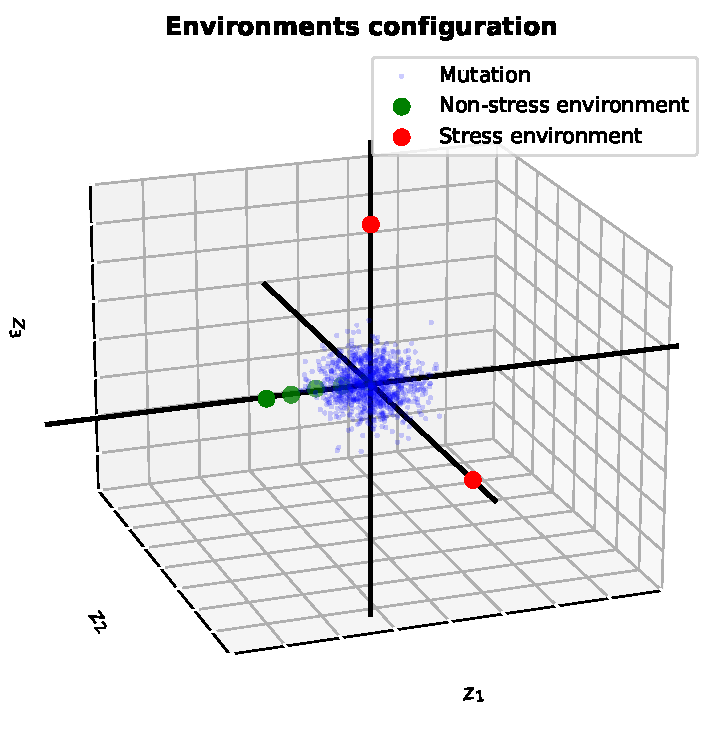
\includegraphics[width=0.99\linewidth]{environment_configuration.pdf}
  \caption{}
  \label{fig:sfig4a}
\end{subfigure}%
\begin{subfigure}{.5\textwidth}
  % \centering
  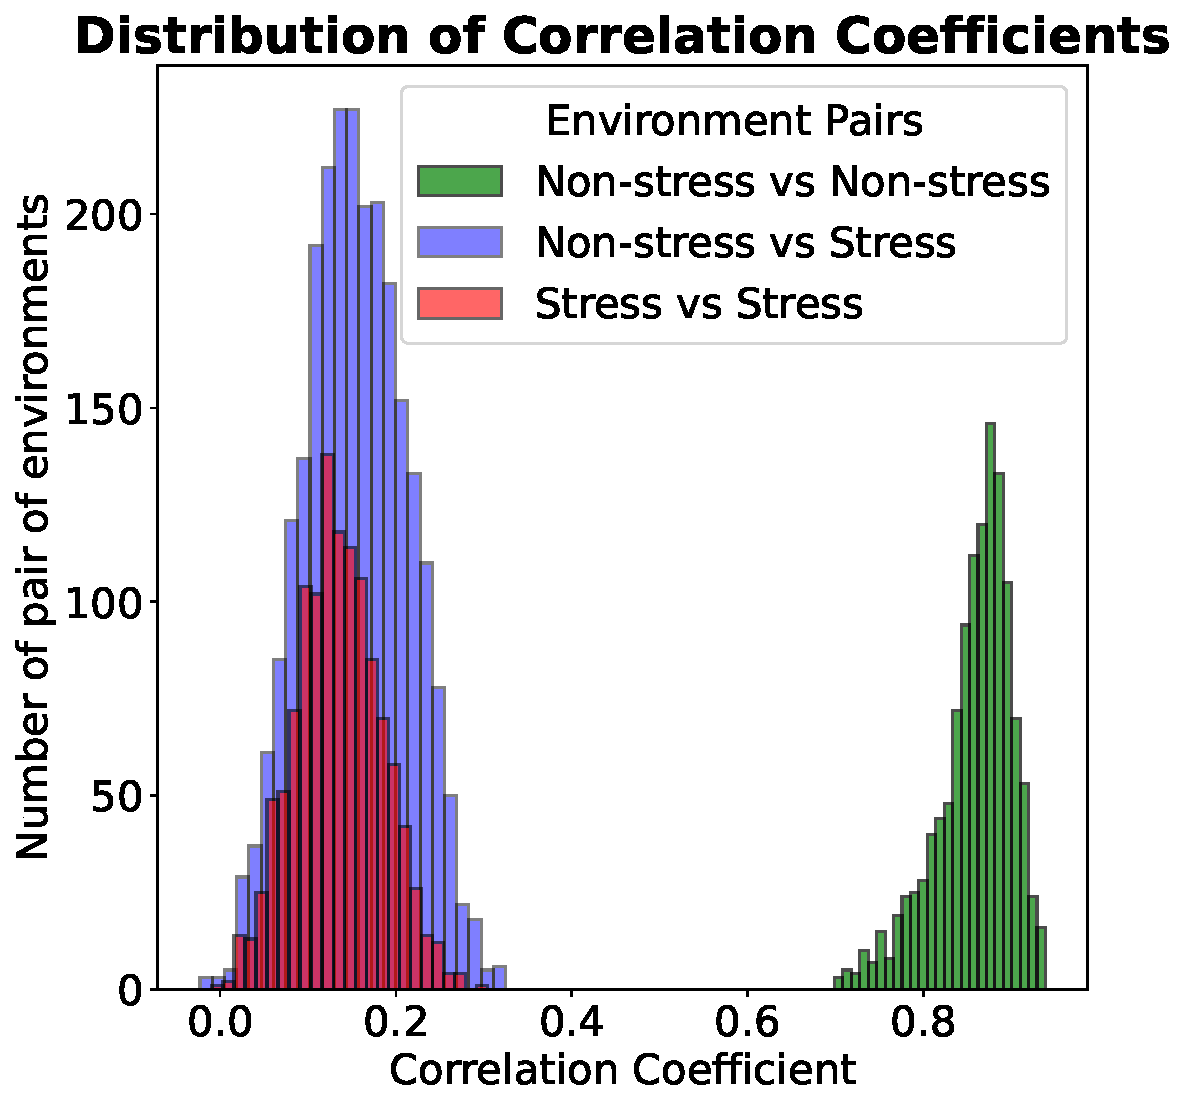
\includegraphics[width=1\linewidth]{correlation_simulation.pdf}
  \caption{}
  \label{fig:sfig4b}
\end{subfigure} \\
\begin{subfigure}{.5\textwidth}
  % \centering
  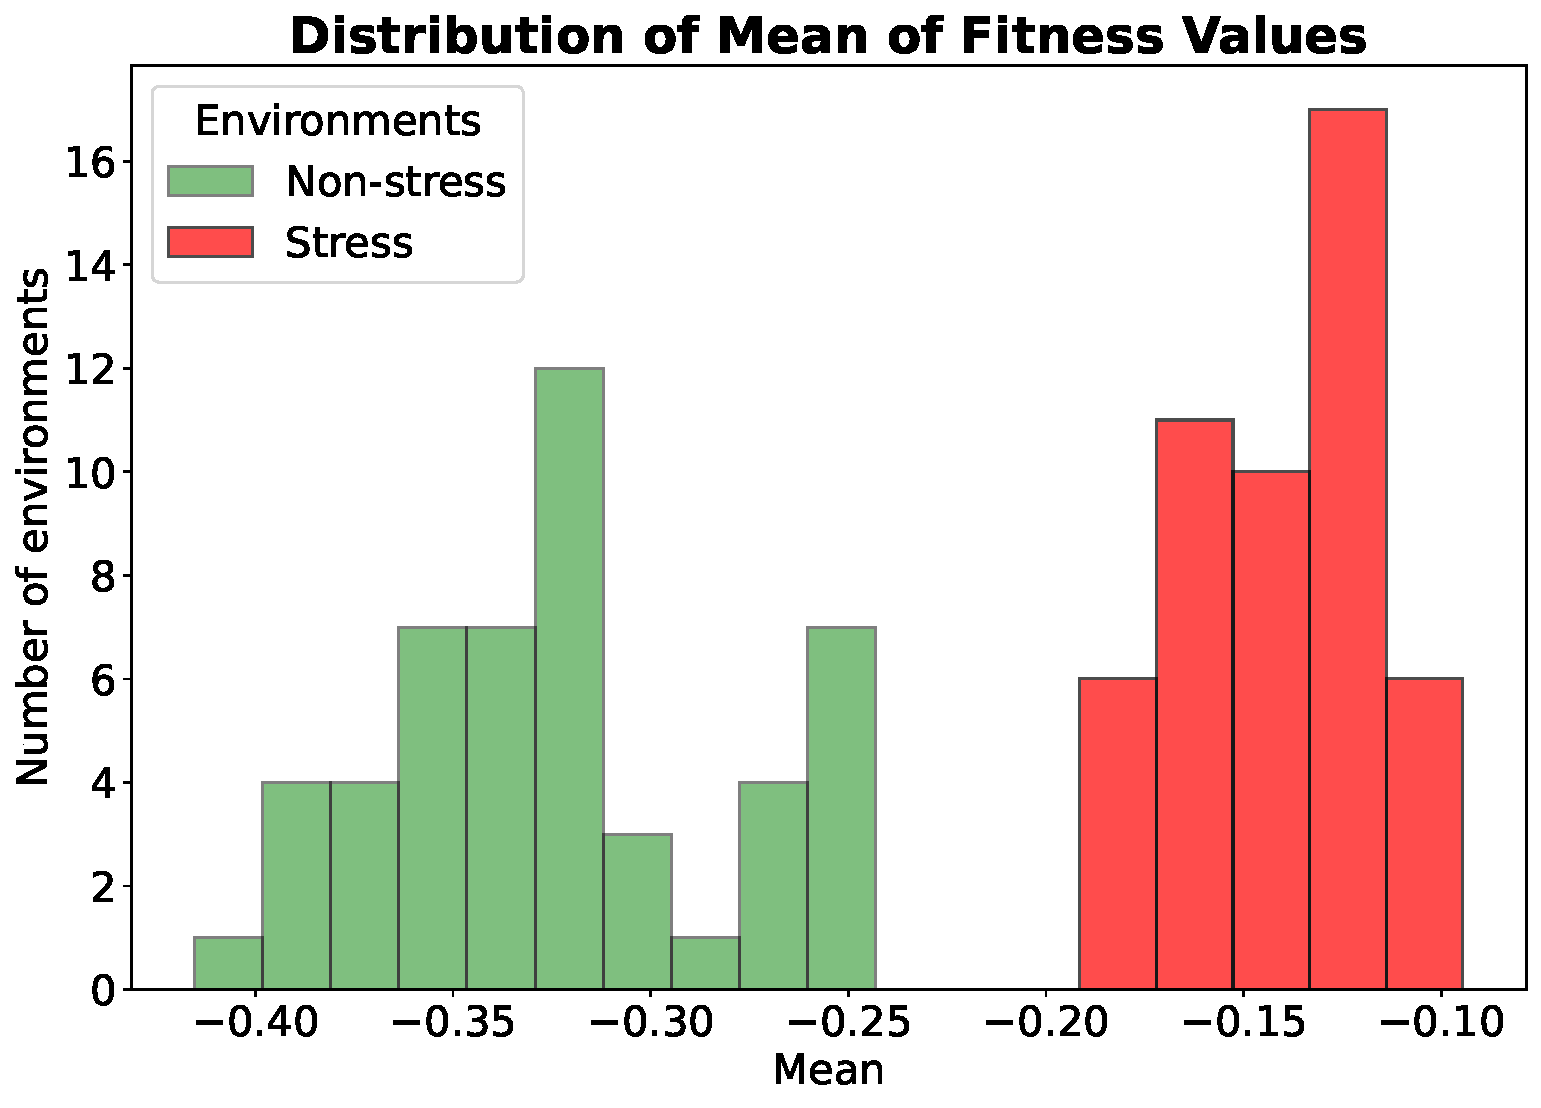
\includegraphics[width=1\linewidth]{mean_simulation.pdf}
  \caption{}
  \label{fig:sfig4c}
\end{subfigure}%
\begin{subfigure}{.5\textwidth}
  % \centering
  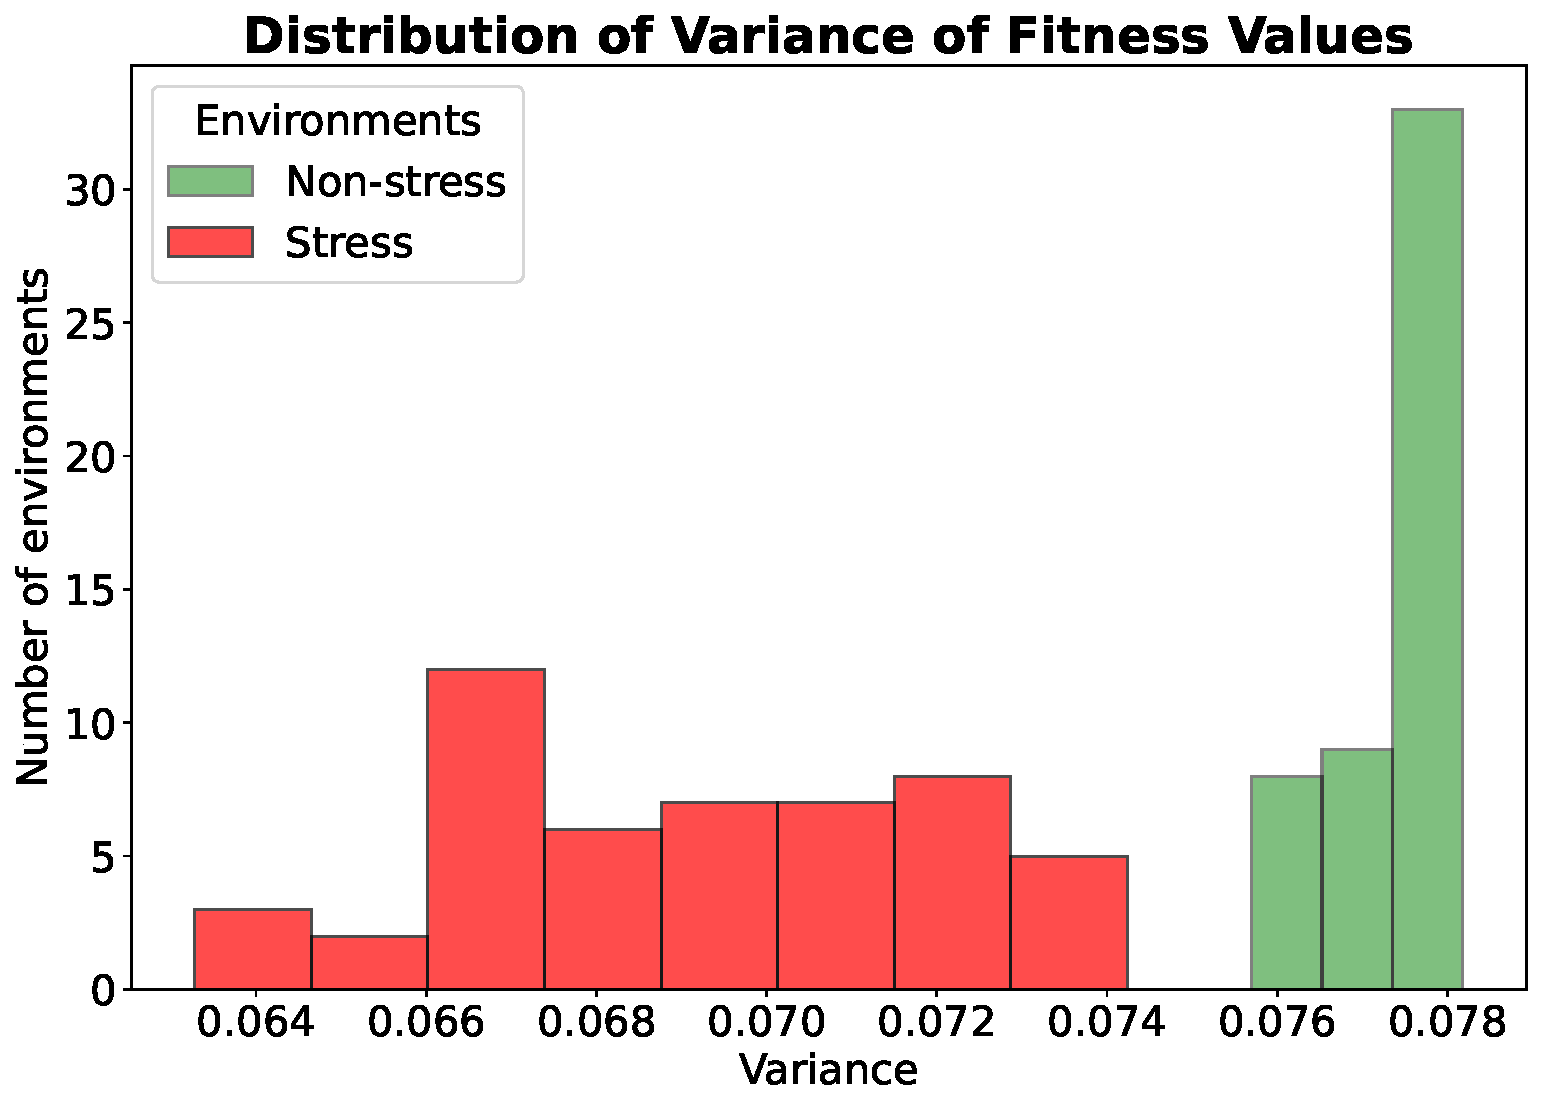
\includegraphics[width=1\linewidth]{standard_deviation_simulation.pdf}
  \caption{}
  \label{fig:sfig4d}
\end{subfigure}
\caption{Figure \ref{fig:sfig4a} is a schematics diagram of the configuration of phenotypic space alongside with ancestor phenotype $\ket{\mathbf{z}_0}$ at the center of the coordinate system, and the blue dots representing  new phenotypes after mutation. The red and green dots signify the phenotypic optimum of stress and non-stress environments, respectively. The simulation was performed using $10,000$ mutants and $100$ environments within a $51$ dimensional phenotypic space, which results in the distribution of mean, variance, and correlation coefficient depicted in the Figure \ref{fig:sfig4c}, \ref{fig:sfig4d}, and \ref{fig:sfig4b}, repectively.}
\label{fig:fig4}
\end{figure}

Figure \ref{fig:sfig4a} shows a cartoon picture of the phenotypic space where the ancestor phenotype $\ket{\mathbf{z}_0}$ is placed in the center of the phenotype space. From the pattern in the experimental data in Figure \ref{fig:sfig3b} we learned that the non-stress environments are alike (having a high correlation with each other), their optima are placed on a single axis. Furthermore, the optimum of each stress environment is placed on all the other perpendicular axes. According to equation (9), this configuration might give us a theoretically calculated distribution of correlation coefficients that is closer to the experimental one. However, since not all the correlation between stress environments and stress vs non-stress environments are not at the same value, we have introduced small noise values to the coordinates of the optima of the environments so that it produces a distribution more like the experimental one.

Moreover, in the last section we established the fact that, if the log-fitness function is more concave around some area, the value of mean is going to be more negative. So, if the neighborhood of environmental optima is more concave than the points far away from the optima, then the ancestor phenotype close to the environmental optima would have a more negative mean, and hence more deletarious mutation would appear in that environment. To test this hypothesis, the optima of stress environments are placed far from the ancestor phenotype, and for non-stress environments, the optima are positioned close to the center of the phenotype space. These placements make sense because if the environment is most suitable for the ancestor, the optimum phenotype of that environment must coincide with the ancestor phenotype. If the optimum phenotype is closer to the ancestor phenotype, it would take a small number of steps to reach a stable situation. However, the opposite would happen with regard to optima being far from the ancestor phenotype.  

In most of the literature, the Gaussian function is used to represent the fitness function, which amounts to using $Q=2, \alpha <0$ in the equation (10). However, this choice would not provide the correct qualitative statistical representation of the data presented in Figure \ref{fig:fig3}. From equation (12), it is very easy to observe that if $Q$ is equal to $2$, the value of the mean $M$ is independent of the distance from the environmental optimum phenotype to the ancestor phenotype $||\mathbf{z}_0 - \zeta_0||$, which contradicts with the experimental result shown in figure \ref{fig:sfig3c}. Moreover, $Q=2$ implies that $V$ would increase as $||\mathbf{z}_0 - \zeta_0||$ increases according to formula (11); it is completely opposite to the behavior displayed in figure \ref{fig:sfig3d}. Hence, we can conclude that traditional FGM with a Gaussian fitness function would not qualitatively reproduce the experimental data. 

To achieve a more accurate qualitative match with the experimental data, we want both $|M|$ and $V$ to decrease as $||\mathbf{z}_0 - \zeta_0||$ increases, despite ${W}(\ket{\mathbf{z}_0},\ket{\mathbf{z}_{\mathrm{opt}}}) = \exp\left(\alpha||\mathbf{z}_0 - \zeta_0||^Q\right)$ to decrease monotonically from the optimum, provided $\alpha <0$. The monotonically decreasing condition can be achieved if $Q$ is positive and according to equations (11) and (12), both $M$ and $V$ would decrease if $Q<1$. Therefore, the suitable choice for $Q$ is just between $0$ to $1$. In Figure \ref{fig:fig4} $Q=1/2$ is used to generate the numerical simulation result for correlation coefficients, mean, and variance of relative fitness values of 50 stress and 50 non-stress environments. The phenotype space is chosen to be 51-dimensional, and all non-stress environments are placed near 50 different orthogonal axes. All stress environments are located along the final axis orthogonal to the other 50 axes. 

Besides these specifications, we used $\sigma_{\mathrm{mut}} = 0.1, \ \alpha = -1$ and, $10,000$ mutation vectors are being used for this simulation. As predicted by the theoretical calculation, in figures \ref{fig:sfig4c} and \ref{fig:sfig4d}, $M$ and $V$ behave as expected; however, we can see there is a clear separation between the values $M$ and $V$ of stress and non-stress environments which is not present in the experimental data. The mean and variances values are more spread out in experimental data compared to numerical simulation ones. It is also very apparent that the values of $V$ in numerical simulation is far off from the experimental results. Furthermore, in Figure \ref{fig:sfig3b} the correlation coefficients between stress environments are more dispersed compared to the simulation in Figure \ref{fig:sfig4b}. There are also several experimental data points exhibiting negative correlations, which are not captured by the simulation results. Overall, the numerical simulation qualitatively reproduces some of the key statistical features of the empirical data. However, a more detailed analysis of the experimental data, and further refinement of the theoretical model are necessary to achieve a more accurate comparison.

\section{Conclusion}
In this work, we have utilized a simple set of assumptions within the Fisher’s Geometric Model  framework to derive theoretical results and, based on these, designed a specific configuration of the phenotypic space with different elements incorporated. Using this configuration, we computed key statistical parameters of the Distribution of Fitness Effects (DFE) and qualitatively compared them with experimental results. While the model successfully captures some features of the empirical data, it fails to account for finer nuances, highlighting its limitations. Additionally, some of our parameter choices were somewhat ad hoc. It may be possible to extract model parameters directly from experimental data, enabling a more concrete and quantitative comparison between the model and empirical observations. For instance, rather than introducing random noise to perturb coordinates, one could use equation (9) to more precisely determine the direction of the environment’s optimum location. Subsequently, equation (12) could be employed to estimate the distance to the optimum based on experimental data. Finally, using these newly acquired coordinates for the environmental optimum, a more accurate numerical comparison could be envisioned by applying equation (11). 

Furthermore, the agreement between the model and empirical data can potentially be improved by revising some of the underlying hypotheses. For example, instead of relying solely on the stabilizing selection hypothesis, one could design a fitness landscape with multiple optima or incorporate a flat region along certain directions. In addition to modeling the environmental optimum, other parameters that vary with the environment could be introduced, allowing the model to distinguish between stress and non-stress environments even when they exhibit similar means and variances. Similarly, relaxing the universal pleiotropy assumption and adopting a more complex probability distribution for the genotype-to-phenotype mapping could yield a richer, more realistic model. In fact, random matrix theory has previously been employed to capture this relationship more effectively \cite{martin2006general}. Nonetheless, the strength of FGM lies in its simplicity, which has enabled it to make insightful predictions across many areas of evolutionary genetics—including the study of DFEs, epistasis, dominance, adaptive trajectories, and the distribution of fixed mutations. Our current analysis indicates that there is still considerable room for refinement; in particular, the emergence of a power-law log-fitness function in our study suggests opportunities to revisit and extend previously established results derived under the Gaussian fitness assumption. Finally, this modeling framework could be applied to other microorganisms as well, offering a way to further investigate how environmental factors shape the distribution of fitness effects.
\bibliographystyle{unsrt}  
\bibliography{references}  %%% Remove comment to use the external .bib file (using bibtex).
%%% and comment out the ``thebibliography'' section.


%%% Comment out this section when you \bibliography{references} is enabled.
% \begin{thebibliography}{1}

% \bibitem{kour2014real}
% George Kour and Raid Saabne.
% \newblock Real-time segmentation of on-line handwritten arabic script.
% \newblock In {\em Frontiers in Handwriting Recognition (ICFHR), 2014 14th
%   International Conference on}, pages 417--422. IEEE, 2014.

% \bibitem{kour2014fast}
% George Kour and Raid Saabne.
% \newblock Fast classification of handwritten on-line arabic characters.
% \newblock In {\em Soft Computing and Pattern Recognition (SoCPaR), 2014 6th
%   International Conference of}, pages 312--318. IEEE, 2014.

% \bibitem{hadash2018estimate}
% Guy Hadash, Einat Kermany, Boaz Carmeli, Ofer Lavi, George Kour, and Alon
%   Jacovi.
% \newblock Estimate and replace: A novel approach to integrating deep neural
%   networks with existing applications.
% \newblock {\em arXiv preprint arXiv:1804.09028}, 2018.

% \end{thebibliography}


\end{document}
